\begin{name}
	{\tenchude}
	{\tendethi}
	{\tentruong}
	{\thoigian}
	\end{name}
\TN
\Opensolutionfile{ans}[ans/de11-phanI]
\begin{ex}%[2D1N2-2]
	Cho hàm số $y=f(x)$ có bảng biến thiên như hình sau:
	\begin{center}
		\begin{tikzpicture}[scale=1, font=\footnotesize, line width=1pt]
			\tkzTabInit[nocadre=true, lgt=1.2, espcl=2, deltacl=0.6]
			{$x$/0.8,$f'(x)$/0.6,$f(x)$/2}
			{$-\infty$,$0$,$2$,$+\infty$};
			\tkzTabLine{,-,$0$,+,$0$,-,};
			\tkzTabVar{+/$+\infty$,-/$1$,+/$5$,-/$-\infty$};
		\end{tikzpicture}
	\end{center}
	Giá trị cực đại của hàm số đã cho bằng
	\choice
	{$0$}
	{$2$}
	{\True $5$}
	{$1$}
	\loigiai
	{
		Từ bảng biến thiên ta có giá trị cực đại của hàm số đã cho bằng $5$ tại $x=2$.
	}
\end{ex}

\begin{ex}%[2H5N3-2]
	Trong không gian $Oxyz$, cho mặt cầu $(S)\colon(x-2)^2+(y+1)^2+(z-3)^2=4$. Tâm của $(S)$ có tọa độ là
	\choice
	{$(-4;2;-6)$}
	{$(-2;1;-3)$}
	{\True $(2;-1;3)$}
	{$(4;-2;6)$}
	\loigiai
	{
		Tâm của $(S)$ có tọa độ là $(2,-1,3)$.
	}
\end{ex}

\begin{ex}%[1D6H4-2]
	Nếu $\log_8p=m$ thì $\log_2p$ bằng
	\choice
	{$\dfrac{m}{3}$}
	{$\dfrac{3}{m}$}
	{$m^3$}
	{\True $3m$}
	\loigiai
	{
		$\log_8p=m \Rightarrow p=8^m \Rightarrow \log_2p=\log_28^m=m\log_28=3m$.
	}
\end{ex}

\begin{ex}%[1H8N1-2]
	Cho hình hộp chữ nhật $ABCD.A'B'C'D'$. Hai đường thẳng nào sau đây vuông góc với nhau?
	\choice
	{$BD$ và $C'D'$}
	{\True $AA'$ và $BD$}
	{$A'B$ và $CD$}
	{$BB'$ và $DD'$}
	\loigiai
	{
		\begin{center}
			\begin{tikzpicture}[scale=1, font=\footnotesize,>=stealth, line width=1pt]%<DTools>
				%Gán số liệu.
				\def\canhAD{3};\def\canhBA{2};\def\gocBAD{-130};\def\h{4};\def\xdinhA'{0};
				%Gán tọa độ.
				\coordinate (A) at (0,0);
				\coordinate (B) at ($(A)+(\gocBAD:\canhBA)$);
				\coordinate (C) at ($(B)+(0:\canhAD)$);
				\coordinate (D) at ($(A)+(0:\canhAD)$);
				\coordinate (A') at ($(A)+(\xdinhA',\h)$);
				\coordinate (B') at ($(B)+(\xdinhA',\h)$);
				\coordinate (C') at ($(C)+(\xdinhA',\h)$);
				\coordinate (D') at ($(D)+(\xdinhA',\h)$);
				%Vẽ khối lẳng trụ ABCD.A'B'C'D'.
				\draw (A')--(B')--(B)--(C)--(C')--(D')--cycle (B')--(C') (D')--(D)--(C);
				\draw[dashed] (A)--(D) (A')--(A)--(B);
				%Gán nhãn.
				\foreach \x/\y in {A/180, B/180, C/0, D/0, A'/180, B'/180, C'/0, D'/0}{\fill (\x) circle(1pt) ($(\x)+(\y:0.3cm)$) node{$\x$};}
			\end{tikzpicture}
		\end{center}
		Ta có $AA'\perp (ABCD) \Rightarrow AA'\perp BD$.
	}
\end{ex}

\begin{ex}%[2D4H1-3]
	Hàm số $F(x)=\sin 2x$ là một nguyên hàm của hàm số nào sau đây?
	\choice
	{$f_3(x)=\cos 2x$}
	{\True $f_2(x)=2\cos 2x$}
	{$f_1(x)=\dfrac{1}{2}\cos 2x$}
	{$f_4(x)=-\dfrac{1}{2}\cos 2x$}
	\loigiai
	{
		Ta có $f(x)=F'(x) =(\sin 2x)'=2\cos 2x$.
	}
\end{ex}

\begin{ex}%[2D1H1-1]
	Hàm số $y=x^4-2x^2+5$ đồng biến trên khoảng nào sau đây?
	\choice
	{$(-\infty;-1)$}
	{$(0;1)$}
	{\True $(-1;0)$}
	{$(0;+\infty)$}
	\loigiai
	{
		Hàm số trên có bảng biến thiên
		\begin{center}
			\begin{tikzpicture}[scale=1, font=\footnotesize, line width=1pt]%<DTools>
				\tkzTabInit[nocadre=true, lgt=1.2, espcl=2, deltacl=0.6]
				{$x$/0.8,$f'(x)$/0.6,$f(x)$/2}
				{$-\infty$,$-1$,$0$,$1$,$+\infty$};
				\tkzTabLine{,-,$0$,+,$0$,-,$0$,+,};
				\tkzTabVar{+/$+\infty$,-/$4$,+/$5$,-/$4$,+/$+\infty$};
			\end{tikzpicture}
		\end{center}
		Từ bảng biến thiên ta thấy hàm số đồng biến trên $(-1;0)$ và $(1;+\infty)$.
	}
\end{ex}

\begin{ex}%[0H5V4-1]
	Cho hình chóp $S.ABC$ có đáy $ABC$ là tam giác đều, $AB=1$, cạnh bên $SB$ vuông góc với mặt phẳng đáy và $SB=1$. Tích vô hướng của hai vectơ $\overrightarrow{SA}$ và $\overrightarrow{SB}$ bằng
	\choice
	{\True $1$}
	{$\sqrt{2}$}
	{$2$}
	{$\dfrac{\sqrt{2}}{2}$}
	\loigiai
	{
		\begin{center}
			\begin{tikzpicture}[scale=1, font=\footnotesize,>=stealth, line width=1pt]%<DTools>
				%Gán số liệu.
				\def\canhBC{4};\def\canhAB{2};\def\gocABC{-50};\def\h{3};\def\xdinhS{0};
				%Gán tọa độ.
				\coordinate (B) at (0,0);
				\coordinate (A) at ($(B)+(\gocABC:\canhAB)$);
				\coordinate (C) at ($(B)+(0:\canhBC)$);
				\coordinate (S) at ($(B)+(\xdinhS,\h)$);
				%Vẽ khối chóp S.BAC.
				\draw (S)--(A) (S)--(B)--(A) (S)--(C)--(A);
				\draw[dashed] (B)--(C);
				%Gán nhãn.
				\foreach \x/\y in {S/90,B/180,A/-90,C/0}{\fill (\x) circle (1pt) ($(\x)+(\y:0.3cm)$) node{$\x$};}
			\end{tikzpicture}
		\end{center}
		$SB\perp (ABC) \Rightarrow SB \perp AB$ mà $SB=AB=1$ nên tam giác $ABC$ là tam giác vuông cân.\\
		Suy ra $\widehat{ASB}=45^\circ$.\\
		Ta có $SA=\sqrt{SB^2+AB^2}=\sqrt{1^2+1^2}=\sqrt{2}$.\\
		Vậy $\overrightarrow{SA}\cdot \overrightarrow{SB}=\left|\overrightarrow{SA}\right|\cdot \left|\overrightarrow{SB}\right|\cdot \cos \widehat{ASB}=\sqrt{2} \cdot 1 \cdot \dfrac{\sqrt{2}}{2}=1$.
	}
\end{ex}

\begin{ex}%[1D2H2-4]
	Cho cấp số cộng $6$, $17$, $28$, $\ldots$, số hạng thứ $10$ của cấp số cộng đã cho bằng
	\choice
	{$108$}
	{$106$}
	{$107$}
	{\True $105$}
	\loigiai
	{
		Cấp số cộng có $u_1=6$ và công sai $d=11$.\\
		Số hạng thứ $10$ là $u_{10}=u_1+(10-1)d=6+9\cdot 11=105$.
	}
\end{ex}

\begin{ex}%[2D4H2-1]
	Nếu $\displaystyle\int\limits_0^2f(x)\mathrm{\, d}x=4$ thì $\displaystyle\int\limits_0^2\left[f(x)-3\right]\mathrm{\, d}x$ bằng
	\choice
	{$-4$}
	{$1$}
	{\True $-2$}
	{$3$}
	\loigiai
	{
		$\displaystyle\int\limits_0^2\left[f(x)-3\right]\mathrm{\, d}x=\displaystyle\int\limits_0^2f(x)\mathrm{\, d}x-\displaystyle\int\limits_0^2 3\mathrm{\, d}x=4-6=-2$.
	}
\end{ex}

\begin{ex}%[2D3N1-4]
	Cân nặng của một số quả mít trong khu vườn được thống kê ở bảng sau
	\begin{center}
		\begin{tabular}{|l|c|c|c|c|c|}
			\hline Cân nặng (kg)&{$[4;6)$}&{$[6;8)$}&{$[8;10)$}&{$[10;12)$}&{$[12;14)$}\\
			\hline Số quả mít&$6$&$12$&$19$&$9$&$4$\\
			\hline
		\end{tabular}
	\end{center}
	Số quả mít có cân nặng ít hơn $10$ kg trong bảng trên là
	\choice
	{$19$}
	{$46$}
	{$40$}
	{\True $37$}
	\loigiai
	{
		Từ bảng số liệu ta có số quả mít có cân nặng ít hơn $10$ kg là $$6+12+19=37.$$
	}
\end{ex}

\begin{ex}%[2H2H2-3]
	Trong không gian $Oxyz$, cho điểm $M(2;0;1)$. Gọi $A$, $B$ lần lượt là hình chiếu vuông góc của $M$ trên trục $O x$ và trên mặt phẳng $(Oyz)$. Đường thẳng $AB$ có một vectơ chỉ phương là vectơ nào sau đây?
	\choice
	{$\vec{u}_1=(2;0;1)$}
	{\True $\vec{u}_2=(-2;0;1)$}
	{$\vec{u}_3=(1;0;-2)$}
	{$\vec{u}_4=(1;0;2)$}
	\loigiai
	{
		$A$ là hình chiếu vuông góc của $M$ trên trục $Ox$ nên $A(2;0;1)$.\\
		$B$ là hình chiếu vuông góc của $M$ trên mặt phẳng $Oyz$ nên $B(0;0;1)$.\\
		Véctơ chỉ phương của đường thẳng $AB$ là véctơ $\overrightarrow{AB}=(-2;0;1)$.
	}
\end{ex}

\begin{ex}%[1D6H4-5]
	Tập nghiệm của bất phương trình $5^{x^2}\le 25^x$ chứa bao nhiêu số nguyên?
	\choice
	{\True $3$}
	{$1$}
	{$2$}
	{$4$}
	\loigiai
	{
		$5^{x^2}\le 25^x \Leftrightarrow x^2 \leq 2x \Leftrightarrow x^2-2x\leq 0 \Leftrightarrow 0\leq x \leq 2$.\\
		Suy ra tập nghiệm của bất phương trình chứa các số nguyên là $0$; $1$; $2$.\\
		Vậy tập nghiệm của bất phương trình chứa ba số nguyên.
	}
\end{ex}
\Closesolutionfile{ans}
%{\fontfamily{qtm}\fontsize{13pt}{2pt}\selectfont\textbf{PHẦN II. Câu trắc nghiệm đúng sai}. Thí sinh trả lời từ câu 1 đến câu 4. Trong mỗi ý \textbf{a)}, \textbf{b)}, \textbf{c)}, \textbf{d)} ở mỗi câu, thí sinh chọn đúng hoặc sai.}
%\setcounter{ex}{0}% Reset lại số đếm câu hỏi
\TNTF
\Opensolutionfile{ans}[ans/de11-phanII]
\begin{ex}%[2D4H1-3]
	Cho hàm số $f(x)=2x-3\cos x$. Gọi $F(x)$ là một nguyên hàm của hàm số $f(x)$ thoả mãn điều kiện $F\left(\dfrac{\pi}{2}\right)=3$.
	\choiceTF
	{\True $F'(x)=2x-3\cos x$}
	{$\displaystyle\int f(x)\mathrm{\, d}x=x^2+3\sin x+C$}
	{\True $F(x)=x^2-3\sin x+6-\dfrac{\pi^2}{4}$}
	{$F(0)=3-\dfrac{\pi^2}{4}$}
	\loigiai{
		\begin{itemchoice}
			\itemch {\bf Đúng}.\\
			$F(x)$ là nguyên hàm của $f(x)$ nên $F'(x)=f(x)=2x-3\cos x$.
			\itemch {\bf Sai}.\\
			$F(x)=\displaystyle\int f(x)\mathrm{\, d}x=\displaystyle\int 2x-3\cos x\mathrm{\, d}x=x^2-3\sin x +C$.
			\itemch {\bf Đúng}.\\
			$F\left(\dfrac{\pi}{2}\right)=3 \Rightarrow 3=\left(\dfrac{\pi}{2}\right)^2-3\sin \left(\dfrac{\pi}{2}\right)+C \Rightarrow C=6-\left(\dfrac{\pi^2}{4}\right)$.\\
			Vậy $F(x)=x^2-3\sin x+6-\dfrac{\pi^2}{4}$
			\itemch {\bf Sai}.\\
			$F(0)=6-\dfrac{\pi^2}{4}$.
		\end{itemchoice}
		
		
		
	}
\end{ex}

%%%%==============HetCau_EX1==============%%%
%%%%==============Cau_EX2==============%%%
\begin{ex} Vào lúc $12$ giờ trưa, tàu $B$ đang nằm ở vị trí $O$, tàu $A$ cách tàu $B$ $12$ km. Tàu $A$ đang di chuyển về phía $O$ với vận tốc $12$ km/h và tiếp tục di chuyển như vậy cả ngày. Tàu $B$ có vận tốc $8$ km/h đang di chuyển theo hướng vuông góc với hướng đi của tàu $A$ và tiếp tục di chuyển như vậy cả ngày. Quãng đường tàu $A$ và tàu $B$ di chuyển được sau $t$ (giờ) (tính từ lúc $12$ giờ trưa lần lượt là $S_A$ và $S_B$.%[1D7V1-4]
	\choiceTF
	{\True $S_A=12t$ (km) và $S_B=8t$ (km)}
	{Khoảng cách giữa $2$ tàu được xác định bởi công thức $S=\sqrt{S_A^2+S_B^2}$ (km)}
	{Lúc $13$ giờ, khoảng cách giữa $2$ tàu bằng $8\sqrt{10}$ (km)}
	{Lúc $13$ giờ, tốc độ thay đổi khoảng cách giữa $2$ tàu bằng $\dfrac{22\sqrt{10}}{5}$ km/h}
	\loigiai{
		\begin{itemchoice}
			\itemch {\bf Đúng}.\\
			Quãng đường tàu $A$ đi được sau $t$ giờ là $S_A=12t$ (km).\\
			Quãng đường tàu $B$ đi được sau $t$ giờ là $S_B=8t$ (km).
			\itemch {\bf Sai}.\\
			Gọi $M$ là vị trí ban đầu của tàu $A$, sau $t$ giờ tàu $A$ đến được vị trí $A$ mới và đi được quãng đường $MA=S_A$, và tàu $B$ đến vị trí $B$ như hình vẽ.
			\begin{center}
				\begin{tikzpicture}[scale=1, font=\footnotesize,line join=round, line cap=round, >=stealth]
					\path
					(0,0) coordinate (O)
					+(-90:3) coordinate (x)
					+(-90:2) coordinate (B)
					+(180:5) coordinate (M)
					+(180:4) coordinate (A)
					;
					\draw[-stealth] (M)--(A);
					\draw[-stealth] (O)--(B);
					\draw (A)--(O)--(x)
					(B)--(A)
					;
					\draw[stealth-stealth] ($(M)+(-90:.3)$)--($(A)+(-90:.3)$) node[midway,below] {$S_A$};
					\draw[stealth-stealth] ($(O)+(0:.5)$)--($(B)+(0:.5)$) node[midway,right] {$S_B$};
					\foreach \x/\g in {M/90,A/90,O/45,B/0}\fill (\x) circle (1pt)+(\g:3mm) node{$\x$};
				\end{tikzpicture}
			\end{center}
			Khoảng cách giữa hai tàu tại thời điểm $t$ là $$S(t)=\sqrt{(12-S_A)^2+S_B^2}=\sqrt{(12-12t)^2+(8t)^2}.$$
			\itemch {\bf Sai}.\\
			Lúc $13$ giờ tàu $B$ cách $O$ một khoảng là $OB=8\cdot 1=8$ (km).\\
			Tàu $A$ cách $O$ một đoạn $OA=12-12=0$ (km).\\
			Vậy khoảng cách giữa hai tàu lúc này chính bằng đoạn $OB=8$ (km).
			\itemch {\bf Sai}.\\
			Ta có
			$S(t)=\sqrt{(12-12t)^2+(8t)^2}=\sqrt{208t^2-288t+144}$.\\
			Vậy $S'(t)=\dfrac{416t-288}{2\sqrt{208t^2-288t+144}}$.\\
			Lúc $13$ giờ ứng với $t=1$ nên ta có
			$S'(1)=\dfrac{32}{2\sqrt{16}}=8$ km/h.
		\end{itemchoice}
		
	}
\end{ex}
%%%==============HetCau_EX2==============%%%
%%%==============Cau_EX3==============%%%
\begin{ex} Một tờ tiền giả lần lượt bị hai người $A$ và $B$ kiểm tra. Xác suất để người $A$ phát hiện ra tờ này giả là $0{,}7$. Nếu người $A$ cho rằng tờ này tiền giả, thì xác suất để người $B$ cũng nhận định như thế là $0{,}8$. Ngược lại, nếu người $A$ cho rằng tờ này là tiền thật thì xác suất để người $B$ cũng nhận định như thế là $0{,}4$.%[2D6V2-3]
	\choiceTF
	{Xác suất để $A$ không phát hiện ra tờ tiền đó giả là $0{,}2$}
	{\True Xác suất để hai người này đều không phát hiện đây là tờ tiền giả là $0{,}12$}
	{\True Xác suất để ít nhất một trong hai người này phát hiện ra tờ tiền đó là giả là $0{,}88$}
	{\True Biết tờ tiền đó đã bị ít nhất một trong hai người này phát hiện là giả, xác suất để $A$ phát hiện ra nó giả là $79{,}5\%$ (làm tròn đến hàng phần chục)}
	\loigiai{
		\begin{itemchoice}
			\itemch {\bf Sai}.\\
			Gọi $A$ là biến cố \lq\lq người $A$ phát hiện tờ tiền này là giả\rq\rq.\\
			Vậy $\overline{A}$ là biến cố \lq\lq người $A$ không phát hiện tờ tiền này là giả\rq\rq.\\
			Gọi $B$ là biến cố \lq\lq người $B$ phát hiện tờ tiền này là giả\rq\rq.\\
			Vậy $\overline{B}$ là biến cố \lq\lq người $B$ không phát hiện tờ tiền này là giả\rq\rq.\\
			Theo đề bài $\mathrm{P}(A)=0{,}7 \Rightarrow \mathrm{P}\left(\overline{A}\right)=1-\mathrm{P}(A)=1-0{,}7=0{,}3$.
			\itemch {\bf Đúng}.\\
			Nếu người $A$ cho rằng tờ tiền này là thật, xác suất để người $B$ cũng nhận định như thế là $\mathrm{P}\left(B\mid\overline{A}\right)=0{,}4$.\\
			Xác suất để cả hai người đều không phát hiện ra tờ tiền giả:
			$$\mathrm{P}\left(\overline{A} \cap\overline{B}\right)=\mathrm{P}(\overline{A}) \cdot \mathrm{P}(B \mid\overline{A})=0{,}3 \cdot 0{,}4=0{,}12.$$
			\itemch {\bf Đúng}.\\
			Gọi $C$ là biến cố \lq\lq Ít nhất một trong hai người này phát hiện ra tờ tiền đó là giả\rq\rq.\\
			Xác suất để ít nhất một trong hai người này phát hiện ra tờ tiền đó là giả là
			$$\mathrm{P}(C)=1-\mathrm{P}\left(\overline{A} \cap\overline{B}\right)=1-0{,}12=0{,}88.$$
			\itemch {\bf Đúng}.\\
			Ta có
			$\mathrm{P}(A \mid C)=\dfrac{\mathrm{P}(C\mid A)\cdot \mathrm{P}(A)}{\mathrm{P}(C)}=\dfrac{1\cdot 0{,}7}{0{,}88}=79{,}5\%$.
		\end{itemchoice}
		
	}
\end{ex}
%%%==============HetCau_EX3==============%%%
%%%==============Cau_EX4==============%%%
\begin{ex}%[2H5V2-8]
	\immini[thm]{
		Một tháp kiểm soát không lưu ở sân bay cao $109$ m đặt một đài kiểm soát không lưu ở độ cao $105$ m. Máy bay trong phạm vi cách đài kiểm soát $450$ km sẽ hiển thị trên màn hình ra đa. Chọn hệ trục tọa độ $Oxyz$ có gốc $O$ trùng với vị trí chân tháp, mặt phẳng ($Oxy$) trùng với mặt đất sao cho trục $Ox$ là hướng Tây, trục $Oy$ là hướng Nam và trục $Oz$ là trục thẳng đứng (Hình vẽ), đơn vị trên mỗi trục là kilômét.
	}
	{
		\tikzset{khongluu/.pic={
				\definecolor{cdce1eb}{RGB}{220,225,235}
				\definecolor{cafb4c8}{RGB}{175,180,200}
				\definecolor{c82d1f5}{RGB}{130,209,245}
				\definecolor{c8ab0e0}{RGB}{138,176,224}
				\definecolor{ce9edf5}{RGB}{233,237,245}
				\definecolor{caaccfa}{RGB}{170,204,250}
				\definecolor{cbec3d2}{RGB}{190,195,210}
				\begin{scope}
					\path[fill=cdce1eb,nonzero rule] (5.13, 5.58) -- (13.02, 5.58) -- (13.02, 0.21) -- (5.13, 0.21) --cycle
					(5.13, 5.58);
					\path[fill=cafb4c8,nonzero rule] (5.13, 5.58) -- (13.02, 5.58) -- (13.02, 4.44) -- (5.13, 4.44) --cycle
					(5.13, 5.58);
					\path[fill=c82d1f5,nonzero rule] (5.14, 4.44) -- (13.03, 4.44) -- (13.03, 3.3) -- (5.14, 3.3) --cycle
					(5.14, 4.44);
					\path[fill=cdce1eb,nonzero rule] (5.13, 5.58) -- (13.02, 5.58) -- (13.02, 0.21) -- (5.13, 0.21) --cycle
					(5.13, 5.58);
					\path[fill=cdce1eb,nonzero rule] (5.13, 5.58) -- (13.02, 5.58) -- (13.02, 4.44) -- (5.13, 4.44) --cycle
					(5.13, 5.58);
					\path[fill=c8ab0e0,nonzero rule] (5.14, 4.44) -- (13.03, 4.44) -- (13.03, 3.3) -- (5.14, 3.3) --cycle
					(5.14, 4.44);
					\path[fill=ce9edf5,nonzero rule] (5.5, 3.3) -- (13.02, 3.3) -- (13.02, 0.7) -- (6.19, 0.7) .. controls (6.17, 0.7) and (6.14, 0.7) ..
					(6.12, 0.7) .. controls (6.1, 0.7) and (6.08, 0.7) ..
					(6.05, 0.71) .. controls (6.03, 0.71) and (6.01, 0.72) ..
					(5.99, 0.73) .. controls (5.97, 0.73) and (5.94, 0.74) ..
					(5.92, 0.75) .. controls (5.9, 0.76) and (5.88, 0.77) ..
					(5.86, 0.78) .. controls (5.84, 0.79) and (5.82, 0.8) ..
					(5.8, 0.81) .. controls (5.79, 0.82) and (5.77, 0.84) ..
					(5.75, 0.85) .. controls (5.73, 0.87) and (5.72, 0.88) ..
					(5.7, 0.9) .. controls (5.68, 0.91) and (5.67, 0.93) ..
					(5.65, 0.95) .. controls (5.64, 0.97) and (5.63, 0.98) ..
					(5.61, 1) .. controls (5.6, 1.02) and (5.59, 1.04) ..
					(5.58, 1.06) .. controls (5.57, 1.08) and (5.56, 1.1) ..
					(5.55, 1.12) .. controls (5.54, 1.14) and (5.53, 1.16) ..
					(5.53, 1.19) .. controls (5.52, 1.21) and (5.52, 1.23) ..
					(5.51, 1.25) .. controls (5.51, 1.27) and (5.5, 1.3) ..
					(5.5, 1.32) .. controls (5.5, 1.34) and (5.5, 1.36) ..
					(5.5, 1.39) --cycle
					(5.5, 3.3);
					\path[fill=ce9edf5,nonzero rule] (13.02, 5.58) -- (13.02, 4.8) -- (6.07, 4.8) .. controls (6.06, 4.8) and (6.04, 4.8) ..
					(6.02, 4.8) .. controls (6, 4.8) and (5.98, 4.8) ..
					(5.96, 4.81) .. controls (5.94, 4.81) and (5.93, 4.82) ..
					(5.91, 4.82) .. controls (5.89, 4.83) and (5.87, 4.83) ..
					(5.85, 4.84) .. controls (5.84, 4.85) and (5.82, 4.86) ..
					(5.8, 4.86) .. controls (5.79, 4.87) and (5.77, 4.88) ..
					(5.75, 4.89) .. controls (5.74, 4.9) and (5.72, 4.92) ..
					(5.71, 4.93) .. controls (5.69, 4.94) and (5.68, 4.95) ..
					(5.67, 4.97) .. controls (5.65, 4.98) and (5.64, 4.99) ..
					(5.63, 5.01) .. controls (5.62, 5.02) and (5.61, 5.04) ..
					(5.6, 5.05) .. controls (5.58, 5.07) and (5.58, 5.08) ..
					(5.57, 5.1) .. controls (5.56, 5.12) and (5.55, 5.13) ..
					(5.54, 5.15) .. controls (5.53, 5.17) and (5.53, 5.19) ..
					(5.52, 5.21) .. controls (5.52, 5.22) and (5.51, 5.24) ..
					(5.51, 5.26) .. controls (5.51, 5.28) and (5.5, 5.3) ..
					(5.5, 5.32) .. controls (5.5, 5.34) and (5.5, 5.35) ..
					(5.5, 5.37) -- (5.5, 5.58) --cycle
					(13.02, 5.58);
					\path[fill=caaccfa,nonzero rule] (13.03, 4.44) -- (13.03, 3.65) -- (6.08, 3.65) .. controls (6.07, 3.65) and (6.05, 3.66) ..
					(6.03, 3.66) .. controls (6.01, 3.66) and (5.99, 3.66) ..
					(5.97, 3.67) .. controls (5.95, 3.67) and (5.94, 3.67) ..
					(5.92, 3.68) .. controls (5.9, 3.69) and (5.88, 3.69) ..
					(5.86, 3.7) .. controls (5.85, 3.71) and (5.83, 3.71) ..
					(5.81, 3.72) .. controls (5.8, 3.73) and (5.78, 3.74) ..
					(5.76, 3.75) .. controls (5.75, 3.76) and (5.73, 3.77) ..
					(5.72, 3.79) .. controls (5.7, 3.8) and (5.69, 3.81) ..
					(5.68, 3.82) .. controls (5.66, 3.84) and (5.65, 3.85) ..
					(5.64, 3.87) .. controls (5.63, 3.88) and (5.62, 3.9) ..
					(5.6, 3.91) .. controls (5.59, 3.93) and (5.58, 3.94) ..
					(5.58, 3.96) .. controls (5.57, 3.98) and (5.56, 3.99) ..
					(5.55, 4.01) .. controls (5.54, 4.03) and (5.54, 4.05) ..
					(5.53, 4.06) .. controls (5.53, 4.08) and (5.52, 4.1) ..
					(5.52, 4.12) .. controls (5.52, 4.14) and (5.51, 4.16) ..
					(5.51, 4.18) .. controls (5.51, 4.19) and (5.51, 4.21) ..
					(5.51, 4.23) -- (5.51, 4.44) --cycle
					(13.03, 4.44);
					\path[fill=cafb4c8,nonzero rule] (11.51, 9.57) -- (10.8, 8.77) .. controls (10.73, 8.77) and (10.21, 8.8) ..
					(9.54, 8.85) -- (10.47, 10.1) -- (10, 10.12) .. controls (9.94, 10.12) and (9.87, 10.11) ..
					(9.81, 10.09) .. controls (9.75, 10.07) and (9.7, 10.04) ..
					(9.65, 9.99) -- (8.48, 8.92) .. controls (8.17, 8.94) and (7.83, 8.96) ..
					(7.72, 8.97) .. controls (7.25, 8.99) and (6.92, 8.5) ..
					(6.92, 8.5) .. controls (6.92, 8.5) and (7.09, 8.09) ..
					(7.54, 8.07) .. controls (7.91, 8.06) and (10, 8.06) ..
					(10.79, 8.06) .. controls (10.84, 8.06) and (10.89, 8.06) ..
					(10.93, 8.07) .. controls (10.98, 8.08) and (11.02, 8.1) ..
					(11.06, 8.12) .. controls (11.1, 8.14) and (11.14, 8.17) ..
					(11.17, 8.2) .. controls (11.21, 8.23) and (11.24, 8.27) ..
					(11.26, 8.31) -- (12.09, 9.54) --cycle
					(11.51, 9.57);
					\path[fill=cbec3d2,nonzero rule] (11, 8.26) .. controls (11.1, 8.26) and (11.2, 8.29) ..
					(11.28, 8.34) -- (12.09, 9.54) -- (11.51, 9.57) -- (10.8, 8.77) .. controls (10.73, 8.77) and (10.21, 8.8) ..
					(9.54, 8.85) -- (10.47, 10.1) -- (10, 10.12) .. controls (9.94, 10.12) and (9.87, 10.11) ..
					(9.81, 10.09) .. controls (9.75, 10.07) and (9.7, 10.04) ..
					(9.65, 9.99) -- (8.48, 8.92) .. controls (8.17, 8.94) and (7.83, 8.96) ..
					(7.71, 8.97) .. controls (7.49, 8.98) and (7.31, 8.87) ..
					(7.17, 8.76) .. controls (7.14, 8.73) and (7.12, 8.71) ..
					(7.12, 8.71) .. controls (7.12, 8.71) and (7.29, 8.29) ..
					(7.75, 8.27) .. controls (8.12, 8.26) and (10.21, 8.26) ..
					(11, 8.26) --cycle
					(11, 8.26);
					\path[fill=cdce1eb,nonzero rule] (11.61, 4.44) -- (11.82, 4.44) -- (11.82, 3.3) -- (11.61, 3.3) --cycle
					(11.61, 4.44);
					\path[fill=cdce1eb,nonzero rule] (10.3, 4.44) -- (10.5, 4.44) -- (10.5, 3.3) -- (10.3, 3.3) --cycle
					(10.3, 4.44);
					\path[fill=cdce1eb,nonzero rule] (8.98, 4.44) -- (9.19, 4.44) -- (9.19, 3.3) -- (8.98, 3.3) --cycle
					(8.98, 4.44);
					\path[fill=cdce1eb,nonzero rule] (7.67, 4.44) -- (7.87, 4.44) -- (7.87, 3.3) -- (7.67, 3.3) --cycle
					(7.67, 4.44);
					\path[fill=cdce1eb,nonzero rule] (6.35, 4.44) -- (6.56, 4.44) -- (6.56, 3.3) -- (6.35, 3.3) --cycle
					(6.35, 4.44);
					\path[fill=cafb4c8,nonzero rule] (2.28, 13.23) .. controls (2.27, 13.23) and (2.25, 13.23) ..
					(2.24, 13.23) .. controls (2.23, 13.22) and (2.21, 13.22) ..
					(2.2, 13.21) .. controls (2.19, 13.21) and (2.18, 13.2) ..
					(2.16, 13.19) .. controls (2.15, 13.19) and (2.14, 13.18) ..
					(2.13, 13.17) .. controls (2.12, 13.16) and (2.11, 13.15) ..
					(2.11, 13.14) .. controls (2.1, 13.13) and (2.09, 13.11) ..
					(2.09, 13.1) .. controls (2.08, 13.09) and (2.08, 13.08) ..
					(2.08, 13.06) .. controls (2.07, 13.05) and (2.07, 13.04) ..
					(2.07, 13.02) -- (2.07, 11.74) -- (2.49, 11.74) -- (2.49, 13.02) .. controls (2.49, 13.04) and (2.48, 13.05) ..
					(2.48, 13.06) .. controls (2.48, 13.08) and (2.48, 13.09) ..
					(2.47, 13.1) .. controls (2.46, 13.11) and (2.46, 13.13) ..
					(2.45, 13.14) .. controls (2.44, 13.15) and (2.43, 13.16) ..
					(2.43, 13.17) .. controls (2.42, 13.18) and (2.41, 13.19) ..
					(2.39, 13.19) .. controls (2.38, 13.2) and (2.37, 13.21) ..
					(2.36, 13.21) .. controls (2.35, 13.22) and (2.33, 13.22) ..
					(2.32, 13.23) .. controls (2.31, 13.23) and (2.29, 13.23) ..
					(2.28, 13.23) --cycle
					(2.28, 13.23);
					\path[fill=cdce1eb,nonzero rule] (3.93, 10.95) -- (3.93, 10.9) -- (0.63, 10.9) -- (0.63, 10.96) .. controls (0.63, 10.98) and (0.63, 11.01) ..
					(0.63, 11.04) .. controls (0.63, 11.06) and (0.64, 11.09) ..
					(0.64, 11.12) .. controls (0.65, 11.14) and (0.65, 11.17) ..
					(0.66, 11.2) .. controls (0.67, 11.22) and (0.68, 11.25) ..
					(0.69, 11.27) .. controls (0.7, 11.3) and (0.71, 11.32) ..
					(0.72, 11.34) .. controls (0.74, 11.37) and (0.75, 11.39) ..
					(0.76, 11.41) .. controls (0.78, 11.44) and (0.79, 11.46) ..
					(0.81, 11.48) .. controls (0.83, 11.5) and (0.85, 11.52) ..
					(0.87, 11.54) .. controls (0.89, 11.56) and (0.91, 11.58) ..
					(0.93, 11.59) .. controls (0.95, 11.61) and (0.97, 11.63) ..
					(0.99, 11.64) .. controls (1.01, 11.66) and (1.04, 11.67) ..
					(1.06, 11.68) .. controls (1.08, 11.69) and (1.11, 11.71) ..
					(1.13, 11.72) .. controls (1.16, 11.73) and (1.18, 11.74) ..
					(1.21, 11.74) .. controls (1.23, 11.75) and (1.26, 11.76) ..
					(1.29, 11.76) .. controls (1.31, 11.77) and (1.34, 11.77) ..
					(1.37, 11.78) .. controls (1.39, 11.78) and (1.42, 11.78) ..
					(1.45, 11.78) -- (3.11, 11.78) .. controls (3.14, 11.78) and (3.16, 11.78) ..
					(3.19, 11.78) .. controls (3.22, 11.77) and (3.24, 11.77) ..
					(3.27, 11.76) .. controls (3.3, 11.76) and (3.32, 11.75) ..
					(3.35, 11.74) .. controls (3.37, 11.74) and (3.4, 11.73) ..
					(3.42, 11.72) .. controls (3.45, 11.71) and (3.47, 11.69) ..
					(3.5, 11.68) .. controls (3.52, 11.67) and (3.54, 11.66) ..
					(3.57, 11.64) .. controls (3.59, 11.63) and (3.61, 11.61) ..
					(3.63, 11.59) .. controls (3.65, 11.58) and (3.67, 11.56) ..
					(3.69, 11.54) .. controls (3.71, 11.52) and (3.73, 11.5) ..
					(3.75, 11.48) .. controls (3.76, 11.46) and (3.78, 11.44) ..
					(3.79, 11.41) .. controls (3.81, 11.39) and (3.82, 11.37) ..
					(3.84, 11.34) .. controls (3.85, 11.32) and (3.86, 11.3) ..
					(3.87, 11.27) .. controls (3.88, 11.25) and (3.89, 11.22) ..
					(3.9, 11.2) .. controls (3.9, 11.17) and (3.91, 11.14) ..
					(3.92, 11.12) .. controls (3.92, 11.09) and (3.93, 11.06) ..
					(3.93, 11.04) .. controls (3.93, 11.01) and (3.93, 10.98) ..
					(3.93, 10.96) --cycle
					(3.93, 10.95);
					\path[fill=ce9edf5,nonzero rule] (3.11, 11.78) -- (1.45, 11.78) .. controls (1.39, 11.78) and (1.34, 11.77) ..
					(1.29, 11.76) .. controls (1.24, 11.7) and (1.21, 11.64) ..
					(1.19, 11.56) .. controls (1.19, 11.55) and (1.18, 11.54) ..
					(1.18, 11.53) .. controls (1.18, 11.52) and (1.18, 11.51) ..
					(1.18, 11.5) .. controls (1.18, 11.48) and (1.18, 11.47) ..
					(1.18, 11.46) .. controls (1.18, 11.45) and (1.18, 11.44) ..
					(1.18, 11.43) .. controls (1.18, 11.42) and (1.18, 11.4) ..
					(1.19, 11.39) .. controls (1.19, 11.38) and (1.19, 11.37) ..
					(1.2, 11.36) .. controls (1.2, 11.35) and (1.21, 11.34) ..
					(1.21, 11.33) .. controls (1.22, 11.32) and (1.22, 11.31) ..
					(1.23, 11.3) .. controls (1.24, 11.29) and (1.25, 11.28) ..
					(1.25, 11.27) .. controls (1.26, 11.27) and (1.27, 11.26) ..
					(1.28, 11.25) .. controls (1.29, 11.24) and (1.3, 11.24) ..
					(1.31, 11.23) .. controls (1.31, 11.22) and (1.32, 11.22) ..
					(1.33, 11.21) .. controls (1.35, 11.21) and (1.36, 11.2) ..
					(1.37, 11.2) .. controls (1.38, 11.19) and (1.39, 11.19) ..
					(1.4, 11.19) .. controls (1.41, 11.19) and (1.42, 11.18) ..
					(1.43, 11.18) .. controls (1.44, 11.18) and (1.46, 11.18) ..
					(1.47, 11.18) -- (3.9, 11.18) .. controls (3.89, 11.22) and (3.87, 11.26) ..
					(3.86, 11.31) .. controls (3.84, 11.35) and (3.81, 11.38) ..
					(3.79, 11.42) .. controls (3.76, 11.46) and (3.74, 11.49) ..
					(3.71, 11.52) .. controls (3.67, 11.56) and (3.64, 11.59) ..
					(3.61, 11.61) .. controls (3.57, 11.64) and (3.53, 11.66) ..
					(3.49, 11.68) .. controls (3.45, 11.7) and (3.41, 11.72) ..
					(3.37, 11.74) .. controls (3.33, 11.75) and (3.29, 11.76) ..
					(3.24, 11.77) .. controls (3.2, 11.78) and (3.15, 11.78) ..
					(3.11, 11.78) --cycle
					(3.11, 11.78);
					\path[fill=cdce1eb,nonzero rule] (0.83, 7.63) .. controls (0.83, 7.63) and (1.41, 6.21) ..
					(1.41, 4.53) -- (1.41, 0.21) -- (3.15, 0.21) -- (3.15, 4.53) .. controls (3.15, 6.21) and (3.73, 7.63) ..
					(3.73, 7.63) -- (3.73, 7.69) -- (0.83, 7.69) --cycle
					(0.83, 7.63);
					\path[fill=ce9edf5,nonzero rule] (1.93, 5.02) -- (1.93, 1.54) .. controls (1.93, 1.51) and (1.93, 1.48) ..
					(1.93, 1.46) .. controls (1.93, 1.43) and (1.94, 1.4) ..
					(1.94, 1.38) .. controls (1.95, 1.35) and (1.95, 1.32) ..
					(1.96, 1.29) .. controls (1.97, 1.27) and (1.98, 1.24) ..
					(1.99, 1.22) .. controls (2, 1.19) and (2.01, 1.17) ..
					(2.03, 1.14) .. controls (2.04, 1.12) and (2.05, 1.09) ..
					(2.07, 1.07) .. controls (2.08, 1.05) and (2.1, 1.03) ..
					(2.12, 1) .. controls (2.14, 0.98) and (2.15, 0.96) ..
					(2.17, 0.94) .. controls (2.19, 0.92) and (2.21, 0.9) ..
					(2.23, 0.89) .. controls (2.26, 0.87) and (2.28, 0.85) ..
					(2.3, 0.84) .. controls (2.32, 0.82) and (2.35, 0.81) ..
					(2.37, 0.8) .. controls (2.4, 0.78) and (2.42, 0.77) ..
					(2.45, 0.76) .. controls (2.47, 0.75) and (2.5, 0.74) ..
					(2.53, 0.73) .. controls (2.55, 0.72) and (2.58, 0.72) ..
					(2.61, 0.71) .. controls (2.63, 0.71) and (2.66, 0.7) ..
					(2.69, 0.7) .. controls (2.71, 0.7) and (2.74, 0.7) ..
					(2.77, 0.7) -- (3.15, 0.7) -- (3.15, 4.53) .. controls (3.15, 6.21) and (3.73, 7.63) ..
					(3.73, 7.63) -- (3.73, 7.69) -- (1.5, 7.69) .. controls (1.67, 7.15) and (1.93, 6.14) ..
					(1.93, 5.02) --cycle
					(1.93, 5.02);
					
					\path[fill=cafb4c8,nonzero rule] (13.02, -0) -- (0.21, -0) .. controls (0.2, -0) and (0.18, 0) ..
					(0.17, 0) .. controls (0.16, 0.01) and (0.15, 0.01) ..
					(0.13, 0.02) .. controls (0.12, 0.02) and (0.11, 0.03) ..
					(0.1, 0.03) .. controls (0.09, 0.04) and (0.08, 0.05) ..
					(0.07, 0.06) .. controls (0.06, 0.07) and (0.05, 0.08) ..
					(0.04, 0.09) .. controls (0.03, 0.1) and (0.03, 0.12) ..
					(0.02, 0.13) .. controls (0.02, 0.14) and (0.01, 0.15) ..
					(0.01, 0.17) .. controls (0.01, 0.18) and (0.01, 0.19) ..
					(0.01, 0.21) .. controls (0.01, 0.22) and (0.01, 0.23) ..
					(0.01, 0.25) .. controls (0.01, 0.26) and (0.02, 0.27) ..
					(0.02, 0.29) .. controls (0.03, 0.3) and (0.03, 0.31) ..
					(0.04, 0.32) .. controls (0.05, 0.33) and (0.06, 0.34) ..
					(0.07, 0.35) .. controls (0.08, 0.36) and (0.09, 0.37) ..
					(0.1, 0.38) .. controls (0.11, 0.39) and (0.12, 0.39) ..
					(0.13, 0.4) .. controls (0.15, 0.4) and (0.16, 0.41) ..
					(0.17, 0.41) .. controls (0.18, 0.41) and (0.2, 0.41) ..
					(0.21, 0.41) -- (13.02, 0.41) .. controls (13.03, 0.41) and (13.04, 0.41) ..
					(13.06, 0.41) .. controls (13.07, 0.41) and (13.08, 0.4) ..
					(13.1, 0.4) .. controls (13.11, 0.39) and (13.12, 0.39) ..
					(13.13, 0.38) .. controls (13.14, 0.37) and (13.15, 0.36) ..
					(13.16, 0.35) .. controls (13.17, 0.34) and (13.18, 0.33) ..
					(13.19, 0.32) .. controls (13.2, 0.31) and (13.2, 0.3) ..
					(13.21, 0.29) .. controls (13.21, 0.27) and (13.22, 0.26) ..
					(13.22, 0.25) .. controls (13.22, 0.23) and (13.22, 0.22) ..
					(13.22, 0.21) .. controls (13.22, 0.19) and (13.22, 0.18) ..
					(13.22, 0.17) .. controls (13.22, 0.15) and (13.21, 0.14) ..
					(13.21, 0.13) .. controls (13.2, 0.12) and (13.2, 0.1) ..
					(13.19, 0.09) .. controls (13.18, 0.08) and (13.17, 0.07) ..
					(13.16, 0.06) .. controls (13.15, 0.05) and (13.14, 0.04) ..
					(13.13, 0.03) .. controls (13.12, 0.03) and (13.11, 0.02) ..
					(13.1, 0.02) .. controls (13.08, 0.01) and (13.07, 0.01) ..
					(13.06, 0) .. controls (13.04, 0) and (13.03, -0) ..
					(13.02, -0) --cycle
					(13.02, -0);
					
					\path[fill=c8ab0e0,nonzero rule] (0.63, 10.95) -- (3.93, 10.95) -- (3.93, 10.09) -- (0.63, 10.09) --cycle
					(0.63, 10.95);
					
					\path[fill=caaccfa,nonzero rule] (1.26, 10.38) -- (3.93, 10.38) -- (3.93, 10.95) -- (1.01, 10.95) -- (1.01, 10.64) .. controls (1.01, 10.62) and (1.01, 10.6) ..
					(1.02, 10.59) .. controls (1.02, 10.57) and (1.02, 10.56) ..
					(1.03, 10.54) .. controls (1.04, 10.53) and (1.04, 10.51) ..
					(1.05, 10.5) .. controls (1.06, 10.48) and (1.07, 10.47) ..
					(1.08, 10.46) .. controls (1.1, 10.45) and (1.11, 10.44) ..
					(1.12, 10.43) .. controls (1.14, 10.42) and (1.15, 10.41) ..
					(1.17, 10.4) .. controls (1.18, 10.4) and (1.2, 10.39) ..
					(1.21, 10.39) .. controls (1.23, 10.39) and (1.25, 10.38) ..
					(1.26, 10.38) --cycle
					(1.26, 10.38);
					
					\path[fill=cdce1eb,nonzero rule] (2.18, 10.96) -- (2.38, 10.96) -- (2.38, 10.08) -- (2.18, 10.08) --cycle
					(2.18, 10.96);
					
					\path[fill=cdce1eb,nonzero rule] (1.35, 10.96) -- (1.56, 10.96) -- (1.56, 10.08) -- (1.35, 10.08) --cycle
					(1.35, 10.96);
					
					\path[fill=cdce1eb,nonzero rule] (3, 10.96) -- (3.21, 10.96) -- (3.21, 10.08) -- (3, 10.08) --cycle
					(3, 10.96);
					
					\path[fill=c8ab0e0,nonzero rule] (0.83, 9.34) -- (3.73, 9.34) -- (3.73, 7.63) -- (0.83, 7.63) --cycle
					(0.83, 9.34);
					
					\path[fill=caaccfa,nonzero rule] (1.61, 7.91) -- (3.73, 7.91) -- (3.73, 9.34) -- (1.25, 9.34) -- (1.25, 8.27) .. controls (1.25, 8.24) and (1.25, 8.22) ..
					(1.26, 8.2) .. controls (1.26, 8.17) and (1.27, 8.15) ..
					(1.28, 8.13) .. controls (1.29, 8.11) and (1.3, 8.09) ..
					(1.31, 8.07) .. controls (1.33, 8.05) and (1.34, 8.03) ..
					(1.36, 8.01) .. controls (1.37, 8) and (1.39, 7.98) ..
					(1.41, 7.97) .. controls (1.43, 7.95) and (1.45, 7.94) ..
					(1.48, 7.93) .. controls (1.5, 7.92) and (1.52, 7.92) ..
					(1.54, 7.91) .. controls (1.57, 7.91) and (1.59, 7.91) ..
					(1.61, 7.91) --cycle
					(1.61, 7.91);
					
					\path[fill=cdce1eb,nonzero rule] (3.73, 8.57) -- (2.38, 8.57) -- (2.38, 9.34) -- (2.18, 9.34) -- (2.18, 8.57) -- (0.83, 8.57) -- (0.83, 8.36) -- (2.18, 8.36) -- (2.18, 7.63) -- (2.38, 7.63) -- (2.38, 8.36) -- (3.73, 8.36) --cycle
					(3.73, 8.57);
					
					\path[fill=cdce1eb,nonzero rule] (0.63, 10.12) -- (3.93, 10.12) .. controls (3.96, 10.12) and (3.99, 10.12) ..
					(4.01, 10.11) .. controls (4.04, 10.11) and (4.07, 10.1) ..
					(4.09, 10.09) .. controls (4.12, 10.08) and (4.14, 10.06) ..
					(4.16, 10.05) .. controls (4.18, 10.03) and (4.21, 10.02) ..
					(4.22, 10) .. controls (4.24, 9.98) and (4.26, 9.96) ..
					(4.28, 9.94) .. controls (4.29, 9.91) and (4.3, 9.89) ..
					(4.31, 9.86) .. controls (4.32, 9.84) and (4.33, 9.81) ..
					(4.34, 9.79) .. controls (4.34, 9.76) and (4.35, 9.73) ..
					(4.35, 9.71) .. controls (4.35, 9.68) and (4.34, 9.65) ..
					(4.34, 9.63) .. controls (4.33, 9.6) and (4.32, 9.57) ..
					(4.31, 9.55) .. controls (4.3, 9.52) and (4.29, 9.5) ..
					(4.28, 9.48) .. controls (4.26, 9.45) and (4.24, 9.43) ..
					(4.22, 9.41) .. controls (4.21, 9.39) and (4.18, 9.38) ..
					(4.16, 9.36) .. controls (4.14, 9.35) and (4.12, 9.33) ..
					(4.09, 9.32) .. controls (4.07, 9.31) and (4.04, 9.31) ..
					(4.01, 9.3) .. controls (3.99, 9.3) and (3.96, 9.29) ..
					(3.93, 9.29) -- (0.63, 9.29) .. controls (0.6, 9.29) and (0.57, 9.3) ..
					(0.54, 9.3) .. controls (0.52, 9.31) and (0.49, 9.31) ..
					(0.47, 9.32) .. controls (0.44, 9.33) and (0.42, 9.35) ..
					(0.4, 9.36) .. controls (0.37, 9.38) and (0.35, 9.39) ..
					(0.33, 9.41) .. controls (0.31, 9.43) and (0.3, 9.45) ..
					(0.28, 9.48) .. controls (0.27, 9.5) and (0.25, 9.52) ..
					(0.24, 9.55) .. controls (0.23, 9.57) and (0.23, 9.6) ..
					(0.22, 9.63) .. controls (0.21, 9.65) and (0.21, 9.68) ..
					(0.21, 9.71) .. controls (0.21, 9.73) and (0.21, 9.76) ..
					(0.22, 9.79) .. controls (0.23, 9.81) and (0.23, 9.84) ..
					(0.24, 9.86) .. controls (0.25, 9.89) and (0.27, 9.91) ..
					(0.28, 9.94) .. controls (0.3, 9.96) and (0.31, 9.98) ..
					(0.33, 10) .. controls (0.35, 10.02) and (0.37, 10.03) ..
					(0.4, 10.05) .. controls (0.42, 10.06) and (0.44, 10.08) ..
					(0.47, 10.09) .. controls (0.49, 10.1) and (0.52, 10.11) ..
					(0.54, 10.11) .. controls (0.57, 10.12) and (0.6, 10.12) ..
					(0.63, 10.12) --cycle
					(0.63, 10.12);
					
					\path[fill=ce9edf5,nonzero rule] (3.93, 10.12) -- (0.63, 10.12) .. controls (0.56, 10.12) and (0.49, 10.1) ..
					(0.43, 10.07) .. controls (0.43, 10.06) and (0.43, 10.04) ..
					(0.42, 10.03) .. controls (0.42, 10.01) and (0.42, 9.99) ..
					(0.42, 9.98) .. controls (0.42, 9.96) and (0.42, 9.95) ..
					(0.42, 9.93) .. controls (0.42, 9.91) and (0.42, 9.9) ..
					(0.43, 9.88) .. controls (0.43, 9.87) and (0.43, 9.85) ..
					(0.44, 9.84) .. controls (0.44, 9.82) and (0.45, 9.81) ..
					(0.45, 9.79) .. controls (0.46, 9.78) and (0.47, 9.76) ..
					(0.48, 9.75) .. controls (0.48, 9.74) and (0.49, 9.72) ..
					(0.5, 9.71) .. controls (0.51, 9.7) and (0.52, 9.68) ..
					(0.53, 9.67) .. controls (0.54, 9.66) and (0.56, 9.65) ..
					(0.57, 9.64) .. controls (0.58, 9.63) and (0.59, 9.62) ..
					(0.61, 9.61) .. controls (0.62, 9.6) and (0.63, 9.6) ..
					(0.65, 9.59) .. controls (0.66, 9.58) and (0.68, 9.58) ..
					(0.69, 9.57) .. controls (0.71, 9.56) and (0.72, 9.56) ..
					(0.74, 9.56) .. controls (0.75, 9.55) and (0.77, 9.55) ..
					(0.78, 9.55) .. controls (0.8, 9.55) and (0.82, 9.55) ..
					(0.83, 9.55) -- (4.14, 9.55) .. controls (4.21, 9.55) and (4.27, 9.56) ..
					(4.33, 9.59) .. controls (4.34, 9.63) and (4.35, 9.67) ..
					(4.35, 9.71) .. controls (4.35, 9.73) and (4.34, 9.76) ..
					(4.34, 9.79) .. controls (4.33, 9.81) and (4.32, 9.84) ..
					(4.31, 9.86) .. controls (4.3, 9.89) and (4.29, 9.91) ..
					(4.28, 9.94) .. controls (4.26, 9.96) and (4.24, 9.98) ..
					(4.22, 10) .. controls (4.21, 10.02) and (4.18, 10.03) ..
					(4.16, 10.05) .. controls (4.14, 10.06) and (4.12, 10.08) ..
					(4.09, 10.09) .. controls (4.07, 10.1) and (4.04, 10.11) ..
					(4.01, 10.11) .. controls (3.99, 10.12) and (3.96, 10.12) ..
					(3.93, 10.12) --cycle
					(3.93, 10.12);
				\end{scope}
		}}
		\begin{tikzpicture}[scale=.7,transform shape]
			\path (0,0) pic[scale=.3]{khongluu};
			\path (.685,0) coordinate (O)
			+(0:4) coordinate (y) node[above] {$y$}
			+(90:5) coordinate (z) node[above] {$z$}
			+(-145:3) coordinate (x) node[above] {$x$}
			;
			\draw[-stealth] (O)--(z);
			\draw[-stealth] (O)--(y);
			\draw[-stealth] (O)--(x);
		\end{tikzpicture}
	}
	Một máy bay đang ở vị trí $A$ cách mặt đất $8$ km, cách $268$ km về phía Đông, $185$ km về phía Nam so với tháp kiểm soát không lưu và đang chuyển động theo đường thẳng $d$ có vectơ chỉ phương là $\overrightarrow{u}=(82;76;0)$ hướng về đài kiểm soát không lưu.
	\choiceTF
	{Vị trí $A$ có tọa độ là $(268;-185;-8)$}
	{\True Đài kiểm soát không lưu có phát hiện được máy bay tại vị trí $A$}
	{\True Phương trình tham số của đường thẳng $d$ là $\heva{&x=-268+82t\\&y=185+76t\\&z=8}$ ($t$ là tham số)}
	{Khoảng cách gần nhất giữa máy bay và đài kiểm soát không lưu là $217{,}98$ km (làm tròn kết quả đến hàng phần trăm)}
	\loigiai{
		\begin{center}
			\tikzset{khongluu/.pic={
					\definecolor{cdce1eb}{RGB}{220,225,235}
					\definecolor{cafb4c8}{RGB}{175,180,200}
					\definecolor{c82d1f5}{RGB}{130,209,245}
					\definecolor{c8ab0e0}{RGB}{138,176,224}
					\definecolor{ce9edf5}{RGB}{233,237,245}
					\definecolor{caaccfa}{RGB}{170,204,250}
					\definecolor{cbec3d2}{RGB}{190,195,210}
					\begin{scope}
						\path[fill=cdce1eb,nonzero rule] (5.13, 5.58) -- (13.02, 5.58) -- (13.02, 0.21) -- (5.13, 0.21) --cycle
						(5.13, 5.58);
						\path[fill=cafb4c8,nonzero rule] (5.13, 5.58) -- (13.02, 5.58) -- (13.02, 4.44) -- (5.13, 4.44) --cycle
						(5.13, 5.58);
						\path[fill=c82d1f5,nonzero rule] (5.14, 4.44) -- (13.03, 4.44) -- (13.03, 3.3) -- (5.14, 3.3) --cycle
						(5.14, 4.44);
						\path[fill=cdce1eb,nonzero rule] (5.13, 5.58) -- (13.02, 5.58) -- (13.02, 0.21) -- (5.13, 0.21) --cycle
						(5.13, 5.58);
						\path[fill=cdce1eb,nonzero rule] (5.13, 5.58) -- (13.02, 5.58) -- (13.02, 4.44) -- (5.13, 4.44) --cycle
						(5.13, 5.58);
						\path[fill=c8ab0e0,nonzero rule] (5.14, 4.44) -- (13.03, 4.44) -- (13.03, 3.3) -- (5.14, 3.3) --cycle
						(5.14, 4.44);
						\path[fill=ce9edf5,nonzero rule] (5.5, 3.3) -- (13.02, 3.3) -- (13.02, 0.7) -- (6.19, 0.7) .. controls (6.17, 0.7) and (6.14, 0.7) ..
						(6.12, 0.7) .. controls (6.1, 0.7) and (6.08, 0.7) ..
						(6.05, 0.71) .. controls (6.03, 0.71) and (6.01, 0.72) ..
						(5.99, 0.73) .. controls (5.97, 0.73) and (5.94, 0.74) ..
						(5.92, 0.75) .. controls (5.9, 0.76) and (5.88, 0.77) ..
						(5.86, 0.78) .. controls (5.84, 0.79) and (5.82, 0.8) ..
						(5.8, 0.81) .. controls (5.79, 0.82) and (5.77, 0.84) ..
						(5.75, 0.85) .. controls (5.73, 0.87) and (5.72, 0.88) ..
						(5.7, 0.9) .. controls (5.68, 0.91) and (5.67, 0.93) ..
						(5.65, 0.95) .. controls (5.64, 0.97) and (5.63, 0.98) ..
						(5.61, 1) .. controls (5.6, 1.02) and (5.59, 1.04) ..
						(5.58, 1.06) .. controls (5.57, 1.08) and (5.56, 1.1) ..
						(5.55, 1.12) .. controls (5.54, 1.14) and (5.53, 1.16) ..
						(5.53, 1.19) .. controls (5.52, 1.21) and (5.52, 1.23) ..
						(5.51, 1.25) .. controls (5.51, 1.27) and (5.5, 1.3) ..
						(5.5, 1.32) .. controls (5.5, 1.34) and (5.5, 1.36) ..
						(5.5, 1.39) --cycle
						(5.5, 3.3);
						\path[fill=ce9edf5,nonzero rule] (13.02, 5.58) -- (13.02, 4.8) -- (6.07, 4.8) .. controls (6.06, 4.8) and (6.04, 4.8) ..
						(6.02, 4.8) .. controls (6, 4.8) and (5.98, 4.8) ..
						(5.96, 4.81) .. controls (5.94, 4.81) and (5.93, 4.82) ..
						(5.91, 4.82) .. controls (5.89, 4.83) and (5.87, 4.83) ..
						(5.85, 4.84) .. controls (5.84, 4.85) and (5.82, 4.86) ..
						(5.8, 4.86) .. controls (5.79, 4.87) and (5.77, 4.88) ..
						(5.75, 4.89) .. controls (5.74, 4.9) and (5.72, 4.92) ..
						(5.71, 4.93) .. controls (5.69, 4.94) and (5.68, 4.95) ..
						(5.67, 4.97) .. controls (5.65, 4.98) and (5.64, 4.99) ..
						(5.63, 5.01) .. controls (5.62, 5.02) and (5.61, 5.04) ..
						(5.6, 5.05) .. controls (5.58, 5.07) and (5.58, 5.08) ..
						(5.57, 5.1) .. controls (5.56, 5.12) and (5.55, 5.13) ..
						(5.54, 5.15) .. controls (5.53, 5.17) and (5.53, 5.19) ..
						(5.52, 5.21) .. controls (5.52, 5.22) and (5.51, 5.24) ..
						(5.51, 5.26) .. controls (5.51, 5.28) and (5.5, 5.3) ..
						(5.5, 5.32) .. controls (5.5, 5.34) and (5.5, 5.35) ..
						(5.5, 5.37) -- (5.5, 5.58) --cycle
						(13.02, 5.58);
						\path[fill=caaccfa,nonzero rule] (13.03, 4.44) -- (13.03, 3.65) -- (6.08, 3.65) .. controls (6.07, 3.65) and (6.05, 3.66) ..
						(6.03, 3.66) .. controls (6.01, 3.66) and (5.99, 3.66) ..
						(5.97, 3.67) .. controls (5.95, 3.67) and (5.94, 3.67) ..
						(5.92, 3.68) .. controls (5.9, 3.69) and (5.88, 3.69) ..
						(5.86, 3.7) .. controls (5.85, 3.71) and (5.83, 3.71) ..
						(5.81, 3.72) .. controls (5.8, 3.73) and (5.78, 3.74) ..
						(5.76, 3.75) .. controls (5.75, 3.76) and (5.73, 3.77) ..
						(5.72, 3.79) .. controls (5.7, 3.8) and (5.69, 3.81) ..
						(5.68, 3.82) .. controls (5.66, 3.84) and (5.65, 3.85) ..
						(5.64, 3.87) .. controls (5.63, 3.88) and (5.62, 3.9) ..
						(5.6, 3.91) .. controls (5.59, 3.93) and (5.58, 3.94) ..
						(5.58, 3.96) .. controls (5.57, 3.98) and (5.56, 3.99) ..
						(5.55, 4.01) .. controls (5.54, 4.03) and (5.54, 4.05) ..
						(5.53, 4.06) .. controls (5.53, 4.08) and (5.52, 4.1) ..
						(5.52, 4.12) .. controls (5.52, 4.14) and (5.51, 4.16) ..
						(5.51, 4.18) .. controls (5.51, 4.19) and (5.51, 4.21) ..
						(5.51, 4.23) -- (5.51, 4.44) --cycle
						(13.03, 4.44);
						\path[fill=cafb4c8,nonzero rule] (11.51, 9.57) -- (10.8, 8.77) .. controls (10.73, 8.77) and (10.21, 8.8) ..
						(9.54, 8.85) -- (10.47, 10.1) -- (10, 10.12) .. controls (9.94, 10.12) and (9.87, 10.11) ..
						(9.81, 10.09) .. controls (9.75, 10.07) and (9.7, 10.04) ..
						(9.65, 9.99) -- (8.48, 8.92) .. controls (8.17, 8.94) and (7.83, 8.96) ..
						(7.72, 8.97) .. controls (7.25, 8.99) and (6.92, 8.5) ..
						(6.92, 8.5) .. controls (6.92, 8.5) and (7.09, 8.09) ..
						(7.54, 8.07) .. controls (7.91, 8.06) and (10, 8.06) ..
						(10.79, 8.06) .. controls (10.84, 8.06) and (10.89, 8.06) ..
						(10.93, 8.07) .. controls (10.98, 8.08) and (11.02, 8.1) ..
						(11.06, 8.12) .. controls (11.1, 8.14) and (11.14, 8.17) ..
						(11.17, 8.2) .. controls (11.21, 8.23) and (11.24, 8.27) ..
						(11.26, 8.31) -- (12.09, 9.54) --cycle
						(11.51, 9.57);
						\path[fill=cbec3d2,nonzero rule] (11, 8.26) .. controls (11.1, 8.26) and (11.2, 8.29) ..
						(11.28, 8.34) -- (12.09, 9.54) -- (11.51, 9.57) -- (10.8, 8.77) .. controls (10.73, 8.77) and (10.21, 8.8) ..
						(9.54, 8.85) -- (10.47, 10.1) -- (10, 10.12) .. controls (9.94, 10.12) and (9.87, 10.11) ..
						(9.81, 10.09) .. controls (9.75, 10.07) and (9.7, 10.04) ..
						(9.65, 9.99) -- (8.48, 8.92) .. controls (8.17, 8.94) and (7.83, 8.96) ..
						(7.71, 8.97) .. controls (7.49, 8.98) and (7.31, 8.87) ..
						(7.17, 8.76) .. controls (7.14, 8.73) and (7.12, 8.71) ..
						(7.12, 8.71) .. controls (7.12, 8.71) and (7.29, 8.29) ..
						(7.75, 8.27) .. controls (8.12, 8.26) and (10.21, 8.26) ..
						(11, 8.26) --cycle
						(11, 8.26);
						\path[fill=cdce1eb,nonzero rule] (11.61, 4.44) -- (11.82, 4.44) -- (11.82, 3.3) -- (11.61, 3.3) --cycle
						(11.61, 4.44);
						\path[fill=cdce1eb,nonzero rule] (10.3, 4.44) -- (10.5, 4.44) -- (10.5, 3.3) -- (10.3, 3.3) --cycle
						(10.3, 4.44);
						\path[fill=cdce1eb,nonzero rule] (8.98, 4.44) -- (9.19, 4.44) -- (9.19, 3.3) -- (8.98, 3.3) --cycle
						(8.98, 4.44);
						\path[fill=cdce1eb,nonzero rule] (7.67, 4.44) -- (7.87, 4.44) -- (7.87, 3.3) -- (7.67, 3.3) --cycle
						(7.67, 4.44);
						\path[fill=cdce1eb,nonzero rule] (6.35, 4.44) -- (6.56, 4.44) -- (6.56, 3.3) -- (6.35, 3.3) --cycle
						(6.35, 4.44);
						\path[fill=cafb4c8,nonzero rule] (2.28, 13.23) .. controls (2.27, 13.23) and (2.25, 13.23) ..
						(2.24, 13.23) .. controls (2.23, 13.22) and (2.21, 13.22) ..
						(2.2, 13.21) .. controls (2.19, 13.21) and (2.18, 13.2) ..
						(2.16, 13.19) .. controls (2.15, 13.19) and (2.14, 13.18) ..
						(2.13, 13.17) .. controls (2.12, 13.16) and (2.11, 13.15) ..
						(2.11, 13.14) .. controls (2.1, 13.13) and (2.09, 13.11) ..
						(2.09, 13.1) .. controls (2.08, 13.09) and (2.08, 13.08) ..
						(2.08, 13.06) .. controls (2.07, 13.05) and (2.07, 13.04) ..
						(2.07, 13.02) -- (2.07, 11.74) -- (2.49, 11.74) -- (2.49, 13.02) .. controls (2.49, 13.04) and (2.48, 13.05) ..
						(2.48, 13.06) .. controls (2.48, 13.08) and (2.48, 13.09) ..
						(2.47, 13.1) .. controls (2.46, 13.11) and (2.46, 13.13) ..
						(2.45, 13.14) .. controls (2.44, 13.15) and (2.43, 13.16) ..
						(2.43, 13.17) .. controls (2.42, 13.18) and (2.41, 13.19) ..
						(2.39, 13.19) .. controls (2.38, 13.2) and (2.37, 13.21) ..
						(2.36, 13.21) .. controls (2.35, 13.22) and (2.33, 13.22) ..
						(2.32, 13.23) .. controls (2.31, 13.23) and (2.29, 13.23) ..
						(2.28, 13.23) --cycle
						(2.28, 13.23);
						\path[fill=cdce1eb,nonzero rule] (3.93, 10.95) -- (3.93, 10.9) -- (0.63, 10.9) -- (0.63, 10.96) .. controls (0.63, 10.98) and (0.63, 11.01) ..
						(0.63, 11.04) .. controls (0.63, 11.06) and (0.64, 11.09) ..
						(0.64, 11.12) .. controls (0.65, 11.14) and (0.65, 11.17) ..
						(0.66, 11.2) .. controls (0.67, 11.22) and (0.68, 11.25) ..
						(0.69, 11.27) .. controls (0.7, 11.3) and (0.71, 11.32) ..
						(0.72, 11.34) .. controls (0.74, 11.37) and (0.75, 11.39) ..
						(0.76, 11.41) .. controls (0.78, 11.44) and (0.79, 11.46) ..
						(0.81, 11.48) .. controls (0.83, 11.5) and (0.85, 11.52) ..
						(0.87, 11.54) .. controls (0.89, 11.56) and (0.91, 11.58) ..
						(0.93, 11.59) .. controls (0.95, 11.61) and (0.97, 11.63) ..
						(0.99, 11.64) .. controls (1.01, 11.66) and (1.04, 11.67) ..
						(1.06, 11.68) .. controls (1.08, 11.69) and (1.11, 11.71) ..
						(1.13, 11.72) .. controls (1.16, 11.73) and (1.18, 11.74) ..
						(1.21, 11.74) .. controls (1.23, 11.75) and (1.26, 11.76) ..
						(1.29, 11.76) .. controls (1.31, 11.77) and (1.34, 11.77) ..
						(1.37, 11.78) .. controls (1.39, 11.78) and (1.42, 11.78) ..
						(1.45, 11.78) -- (3.11, 11.78) .. controls (3.14, 11.78) and (3.16, 11.78) ..
						(3.19, 11.78) .. controls (3.22, 11.77) and (3.24, 11.77) ..
						(3.27, 11.76) .. controls (3.3, 11.76) and (3.32, 11.75) ..
						(3.35, 11.74) .. controls (3.37, 11.74) and (3.4, 11.73) ..
						(3.42, 11.72) .. controls (3.45, 11.71) and (3.47, 11.69) ..
						(3.5, 11.68) .. controls (3.52, 11.67) and (3.54, 11.66) ..
						(3.57, 11.64) .. controls (3.59, 11.63) and (3.61, 11.61) ..
						(3.63, 11.59) .. controls (3.65, 11.58) and (3.67, 11.56) ..
						(3.69, 11.54) .. controls (3.71, 11.52) and (3.73, 11.5) ..
						(3.75, 11.48) .. controls (3.76, 11.46) and (3.78, 11.44) ..
						(3.79, 11.41) .. controls (3.81, 11.39) and (3.82, 11.37) ..
						(3.84, 11.34) .. controls (3.85, 11.32) and (3.86, 11.3) ..
						(3.87, 11.27) .. controls (3.88, 11.25) and (3.89, 11.22) ..
						(3.9, 11.2) .. controls (3.9, 11.17) and (3.91, 11.14) ..
						(3.92, 11.12) .. controls (3.92, 11.09) and (3.93, 11.06) ..
						(3.93, 11.04) .. controls (3.93, 11.01) and (3.93, 10.98) ..
						(3.93, 10.96) --cycle
						(3.93, 10.95);
						\path[fill=ce9edf5,nonzero rule] (3.11, 11.78) -- (1.45, 11.78) .. controls (1.39, 11.78) and (1.34, 11.77) ..
						(1.29, 11.76) .. controls (1.24, 11.7) and (1.21, 11.64) ..
						(1.19, 11.56) .. controls (1.19, 11.55) and (1.18, 11.54) ..
						(1.18, 11.53) .. controls (1.18, 11.52) and (1.18, 11.51) ..
						(1.18, 11.5) .. controls (1.18, 11.48) and (1.18, 11.47) ..
						(1.18, 11.46) .. controls (1.18, 11.45) and (1.18, 11.44) ..
						(1.18, 11.43) .. controls (1.18, 11.42) and (1.18, 11.4) ..
						(1.19, 11.39) .. controls (1.19, 11.38) and (1.19, 11.37) ..
						(1.2, 11.36) .. controls (1.2, 11.35) and (1.21, 11.34) ..
						(1.21, 11.33) .. controls (1.22, 11.32) and (1.22, 11.31) ..
						(1.23, 11.3) .. controls (1.24, 11.29) and (1.25, 11.28) ..
						(1.25, 11.27) .. controls (1.26, 11.27) and (1.27, 11.26) ..
						(1.28, 11.25) .. controls (1.29, 11.24) and (1.3, 11.24) ..
						(1.31, 11.23) .. controls (1.31, 11.22) and (1.32, 11.22) ..
						(1.33, 11.21) .. controls (1.35, 11.21) and (1.36, 11.2) ..
						(1.37, 11.2) .. controls (1.38, 11.19) and (1.39, 11.19) ..
						(1.4, 11.19) .. controls (1.41, 11.19) and (1.42, 11.18) ..
						(1.43, 11.18) .. controls (1.44, 11.18) and (1.46, 11.18) ..
						(1.47, 11.18) -- (3.9, 11.18) .. controls (3.89, 11.22) and (3.87, 11.26) ..
						(3.86, 11.31) .. controls (3.84, 11.35) and (3.81, 11.38) ..
						(3.79, 11.42) .. controls (3.76, 11.46) and (3.74, 11.49) ..
						(3.71, 11.52) .. controls (3.67, 11.56) and (3.64, 11.59) ..
						(3.61, 11.61) .. controls (3.57, 11.64) and (3.53, 11.66) ..
						(3.49, 11.68) .. controls (3.45, 11.7) and (3.41, 11.72) ..
						(3.37, 11.74) .. controls (3.33, 11.75) and (3.29, 11.76) ..
						(3.24, 11.77) .. controls (3.2, 11.78) and (3.15, 11.78) ..
						(3.11, 11.78) --cycle
						(3.11, 11.78);
						\path[fill=cdce1eb,nonzero rule] (0.83, 7.63) .. controls (0.83, 7.63) and (1.41, 6.21) ..
						(1.41, 4.53) -- (1.41, 0.21) -- (3.15, 0.21) -- (3.15, 4.53) .. controls (3.15, 6.21) and (3.73, 7.63) ..
						(3.73, 7.63) -- (3.73, 7.69) -- (0.83, 7.69) --cycle
						(0.83, 7.63);
						\path[fill=ce9edf5,nonzero rule] (1.93, 5.02) -- (1.93, 1.54) .. controls (1.93, 1.51) and (1.93, 1.48) ..
						(1.93, 1.46) .. controls (1.93, 1.43) and (1.94, 1.4) ..
						(1.94, 1.38) .. controls (1.95, 1.35) and (1.95, 1.32) ..
						(1.96, 1.29) .. controls (1.97, 1.27) and (1.98, 1.24) ..
						(1.99, 1.22) .. controls (2, 1.19) and (2.01, 1.17) ..
						(2.03, 1.14) .. controls (2.04, 1.12) and (2.05, 1.09) ..
						(2.07, 1.07) .. controls (2.08, 1.05) and (2.1, 1.03) ..
						(2.12, 1) .. controls (2.14, 0.98) and (2.15, 0.96) ..
						(2.17, 0.94) .. controls (2.19, 0.92) and (2.21, 0.9) ..
						(2.23, 0.89) .. controls (2.26, 0.87) and (2.28, 0.85) ..
						(2.3, 0.84) .. controls (2.32, 0.82) and (2.35, 0.81) ..
						(2.37, 0.8) .. controls (2.4, 0.78) and (2.42, 0.77) ..
						(2.45, 0.76) .. controls (2.47, 0.75) and (2.5, 0.74) ..
						(2.53, 0.73) .. controls (2.55, 0.72) and (2.58, 0.72) ..
						(2.61, 0.71) .. controls (2.63, 0.71) and (2.66, 0.7) ..
						(2.69, 0.7) .. controls (2.71, 0.7) and (2.74, 0.7) ..
						(2.77, 0.7) -- (3.15, 0.7) -- (3.15, 4.53) .. controls (3.15, 6.21) and (3.73, 7.63) ..
						(3.73, 7.63) -- (3.73, 7.69) -- (1.5, 7.69) .. controls (1.67, 7.15) and (1.93, 6.14) ..
						(1.93, 5.02) --cycle
						(1.93, 5.02);
						
						\path[fill=cafb4c8,nonzero rule] (13.02, -0) -- (0.21, -0) .. controls (0.2, -0) and (0.18, 0) ..
						(0.17, 0) .. controls (0.16, 0.01) and (0.15, 0.01) ..
						(0.13, 0.02) .. controls (0.12, 0.02) and (0.11, 0.03) ..
						(0.1, 0.03) .. controls (0.09, 0.04) and (0.08, 0.05) ..
						(0.07, 0.06) .. controls (0.06, 0.07) and (0.05, 0.08) ..
						(0.04, 0.09) .. controls (0.03, 0.1) and (0.03, 0.12) ..
						(0.02, 0.13) .. controls (0.02, 0.14) and (0.01, 0.15) ..
						(0.01, 0.17) .. controls (0.01, 0.18) and (0.01, 0.19) ..
						(0.01, 0.21) .. controls (0.01, 0.22) and (0.01, 0.23) ..
						(0.01, 0.25) .. controls (0.01, 0.26) and (0.02, 0.27) ..
						(0.02, 0.29) .. controls (0.03, 0.3) and (0.03, 0.31) ..
						(0.04, 0.32) .. controls (0.05, 0.33) and (0.06, 0.34) ..
						(0.07, 0.35) .. controls (0.08, 0.36) and (0.09, 0.37) ..
						(0.1, 0.38) .. controls (0.11, 0.39) and (0.12, 0.39) ..
						(0.13, 0.4) .. controls (0.15, 0.4) and (0.16, 0.41) ..
						(0.17, 0.41) .. controls (0.18, 0.41) and (0.2, 0.41) ..
						(0.21, 0.41) -- (13.02, 0.41) .. controls (13.03, 0.41) and (13.04, 0.41) ..
						(13.06, 0.41) .. controls (13.07, 0.41) and (13.08, 0.4) ..
						(13.1, 0.4) .. controls (13.11, 0.39) and (13.12, 0.39) ..
						(13.13, 0.38) .. controls (13.14, 0.37) and (13.15, 0.36) ..
						(13.16, 0.35) .. controls (13.17, 0.34) and (13.18, 0.33) ..
						(13.19, 0.32) .. controls (13.2, 0.31) and (13.2, 0.3) ..
						(13.21, 0.29) .. controls (13.21, 0.27) and (13.22, 0.26) ..
						(13.22, 0.25) .. controls (13.22, 0.23) and (13.22, 0.22) ..
						(13.22, 0.21) .. controls (13.22, 0.19) and (13.22, 0.18) ..
						(13.22, 0.17) .. controls (13.22, 0.15) and (13.21, 0.14) ..
						(13.21, 0.13) .. controls (13.2, 0.12) and (13.2, 0.1) ..
						(13.19, 0.09) .. controls (13.18, 0.08) and (13.17, 0.07) ..
						(13.16, 0.06) .. controls (13.15, 0.05) and (13.14, 0.04) ..
						(13.13, 0.03) .. controls (13.12, 0.03) and (13.11, 0.02) ..
						(13.1, 0.02) .. controls (13.08, 0.01) and (13.07, 0.01) ..
						(13.06, 0) .. controls (13.04, 0) and (13.03, -0) ..
						(13.02, -0) --cycle
						(13.02, -0);
						
						\path[fill=c8ab0e0,nonzero rule] (0.63, 10.95) -- (3.93, 10.95) -- (3.93, 10.09) -- (0.63, 10.09) --cycle
						(0.63, 10.95);
						
						\path[fill=caaccfa,nonzero rule] (1.26, 10.38) -- (3.93, 10.38) -- (3.93, 10.95) -- (1.01, 10.95) -- (1.01, 10.64) .. controls (1.01, 10.62) and (1.01, 10.6) ..
						(1.02, 10.59) .. controls (1.02, 10.57) and (1.02, 10.56) ..
						(1.03, 10.54) .. controls (1.04, 10.53) and (1.04, 10.51) ..
						(1.05, 10.5) .. controls (1.06, 10.48) and (1.07, 10.47) ..
						(1.08, 10.46) .. controls (1.1, 10.45) and (1.11, 10.44) ..
						(1.12, 10.43) .. controls (1.14, 10.42) and (1.15, 10.41) ..
						(1.17, 10.4) .. controls (1.18, 10.4) and (1.2, 10.39) ..
						(1.21, 10.39) .. controls (1.23, 10.39) and (1.25, 10.38) ..
						(1.26, 10.38) --cycle
						(1.26, 10.38);
						
						\path[fill=cdce1eb,nonzero rule] (2.18, 10.96) -- (2.38, 10.96) -- (2.38, 10.08) -- (2.18, 10.08) --cycle
						(2.18, 10.96);
						
						\path[fill=cdce1eb,nonzero rule] (1.35, 10.96) -- (1.56, 10.96) -- (1.56, 10.08) -- (1.35, 10.08) --cycle
						(1.35, 10.96);
						
						\path[fill=cdce1eb,nonzero rule] (3, 10.96) -- (3.21, 10.96) -- (3.21, 10.08) -- (3, 10.08) --cycle
						(3, 10.96);
						
						\path[fill=c8ab0e0,nonzero rule] (0.83, 9.34) -- (3.73, 9.34) -- (3.73, 7.63) -- (0.83, 7.63) --cycle
						(0.83, 9.34);
						
						\path[fill=caaccfa,nonzero rule] (1.61, 7.91) -- (3.73, 7.91) -- (3.73, 9.34) -- (1.25, 9.34) -- (1.25, 8.27) .. controls (1.25, 8.24) and (1.25, 8.22) ..
						(1.26, 8.2) .. controls (1.26, 8.17) and (1.27, 8.15) ..
						(1.28, 8.13) .. controls (1.29, 8.11) and (1.3, 8.09) ..
						(1.31, 8.07) .. controls (1.33, 8.05) and (1.34, 8.03) ..
						(1.36, 8.01) .. controls (1.37, 8) and (1.39, 7.98) ..
						(1.41, 7.97) .. controls (1.43, 7.95) and (1.45, 7.94) ..
						(1.48, 7.93) .. controls (1.5, 7.92) and (1.52, 7.92) ..
						(1.54, 7.91) .. controls (1.57, 7.91) and (1.59, 7.91) ..
						(1.61, 7.91) --cycle
						(1.61, 7.91);
						
						\path[fill=cdce1eb,nonzero rule] (3.73, 8.57) -- (2.38, 8.57) -- (2.38, 9.34) -- (2.18, 9.34) -- (2.18, 8.57) -- (0.83, 8.57) -- (0.83, 8.36) -- (2.18, 8.36) -- (2.18, 7.63) -- (2.38, 7.63) -- (2.38, 8.36) -- (3.73, 8.36) --cycle
						(3.73, 8.57);
						
						\path[fill=cdce1eb,nonzero rule] (0.63, 10.12) -- (3.93, 10.12) .. controls (3.96, 10.12) and (3.99, 10.12) ..
						(4.01, 10.11) .. controls (4.04, 10.11) and (4.07, 10.1) ..
						(4.09, 10.09) .. controls (4.12, 10.08) and (4.14, 10.06) ..
						(4.16, 10.05) .. controls (4.18, 10.03) and (4.21, 10.02) ..
						(4.22, 10) .. controls (4.24, 9.98) and (4.26, 9.96) ..
						(4.28, 9.94) .. controls (4.29, 9.91) and (4.3, 9.89) ..
						(4.31, 9.86) .. controls (4.32, 9.84) and (4.33, 9.81) ..
						(4.34, 9.79) .. controls (4.34, 9.76) and (4.35, 9.73) ..
						(4.35, 9.71) .. controls (4.35, 9.68) and (4.34, 9.65) ..
						(4.34, 9.63) .. controls (4.33, 9.6) and (4.32, 9.57) ..
						(4.31, 9.55) .. controls (4.3, 9.52) and (4.29, 9.5) ..
						(4.28, 9.48) .. controls (4.26, 9.45) and (4.24, 9.43) ..
						(4.22, 9.41) .. controls (4.21, 9.39) and (4.18, 9.38) ..
						(4.16, 9.36) .. controls (4.14, 9.35) and (4.12, 9.33) ..
						(4.09, 9.32) .. controls (4.07, 9.31) and (4.04, 9.31) ..
						(4.01, 9.3) .. controls (3.99, 9.3) and (3.96, 9.29) ..
						(3.93, 9.29) -- (0.63, 9.29) .. controls (0.6, 9.29) and (0.57, 9.3) ..
						(0.54, 9.3) .. controls (0.52, 9.31) and (0.49, 9.31) ..
						(0.47, 9.32) .. controls (0.44, 9.33) and (0.42, 9.35) ..
						(0.4, 9.36) .. controls (0.37, 9.38) and (0.35, 9.39) ..
						(0.33, 9.41) .. controls (0.31, 9.43) and (0.3, 9.45) ..
						(0.28, 9.48) .. controls (0.27, 9.5) and (0.25, 9.52) ..
						(0.24, 9.55) .. controls (0.23, 9.57) and (0.23, 9.6) ..
						(0.22, 9.63) .. controls (0.21, 9.65) and (0.21, 9.68) ..
						(0.21, 9.71) .. controls (0.21, 9.73) and (0.21, 9.76) ..
						(0.22, 9.79) .. controls (0.23, 9.81) and (0.23, 9.84) ..
						(0.24, 9.86) .. controls (0.25, 9.89) and (0.27, 9.91) ..
						(0.28, 9.94) .. controls (0.3, 9.96) and (0.31, 9.98) ..
						(0.33, 10) .. controls (0.35, 10.02) and (0.37, 10.03) ..
						(0.4, 10.05) .. controls (0.42, 10.06) and (0.44, 10.08) ..
						(0.47, 10.09) .. controls (0.49, 10.1) and (0.52, 10.11) ..
						(0.54, 10.11) .. controls (0.57, 10.12) and (0.6, 10.12) ..
						(0.63, 10.12) --cycle
						(0.63, 10.12);
						
						\path[fill=ce9edf5,nonzero rule] (3.93, 10.12) -- (0.63, 10.12) .. controls (0.56, 10.12) and (0.49, 10.1) ..
						(0.43, 10.07) .. controls (0.43, 10.06) and (0.43, 10.04) ..
						(0.42, 10.03) .. controls (0.42, 10.01) and (0.42, 9.99) ..
						(0.42, 9.98) .. controls (0.42, 9.96) and (0.42, 9.95) ..
						(0.42, 9.93) .. controls (0.42, 9.91) and (0.42, 9.9) ..
						(0.43, 9.88) .. controls (0.43, 9.87) and (0.43, 9.85) ..
						(0.44, 9.84) .. controls (0.44, 9.82) and (0.45, 9.81) ..
						(0.45, 9.79) .. controls (0.46, 9.78) and (0.47, 9.76) ..
						(0.48, 9.75) .. controls (0.48, 9.74) and (0.49, 9.72) ..
						(0.5, 9.71) .. controls (0.51, 9.7) and (0.52, 9.68) ..
						(0.53, 9.67) .. controls (0.54, 9.66) and (0.56, 9.65) ..
						(0.57, 9.64) .. controls (0.58, 9.63) and (0.59, 9.62) ..
						(0.61, 9.61) .. controls (0.62, 9.6) and (0.63, 9.6) ..
						(0.65, 9.59) .. controls (0.66, 9.58) and (0.68, 9.58) ..
						(0.69, 9.57) .. controls (0.71, 9.56) and (0.72, 9.56) ..
						(0.74, 9.56) .. controls (0.75, 9.55) and (0.77, 9.55) ..
						(0.78, 9.55) .. controls (0.8, 9.55) and (0.82, 9.55) ..
						(0.83, 9.55) -- (4.14, 9.55) .. controls (4.21, 9.55) and (4.27, 9.56) ..
						(4.33, 9.59) .. controls (4.34, 9.63) and (4.35, 9.67) ..
						(4.35, 9.71) .. controls (4.35, 9.73) and (4.34, 9.76) ..
						(4.34, 9.79) .. controls (4.33, 9.81) and (4.32, 9.84) ..
						(4.31, 9.86) .. controls (4.3, 9.89) and (4.29, 9.91) ..
						(4.28, 9.94) .. controls (4.26, 9.96) and (4.24, 9.98) ..
						(4.22, 10) .. controls (4.21, 10.02) and (4.18, 10.03) ..
						(4.16, 10.05) .. controls (4.14, 10.06) and (4.12, 10.08) ..
						(4.09, 10.09) .. controls (4.07, 10.1) and (4.04, 10.11) ..
						(4.01, 10.11) .. controls (3.99, 10.12) and (3.96, 10.12) ..
						(3.93, 10.12) --cycle
						(3.93, 10.12);
					\end{scope}
			}}
			\begin{tikzpicture}[scale=.7,transform shape]
				\path (0,0) pic[scale=.3]{khongluu};
				\path (.685,0) coordinate (O) node[below right] {$O$}
				+(0:4) coordinate (y) node[below] {$y$ (Hướng Nam)}
				+(90:5) coordinate (z) node[above] {$z$}
				+(-145:3) coordinate (x) node[below] {$x$ (Hướng Tây)}
				;
				\draw[-stealth] (O)--(z);
				\draw[-stealth] (O)--(y);
				\draw[-stealth] (O)--(x);
			\end{tikzpicture}
		\end{center}
		\begin{itemchoice}
			\itemch {\bf Sai}.\\
			Vị trí $A$ cách mặt đất $8$ km, cách $268$ km về phía Đông, $185$ km về phía Nam nên ta có $A\left(-268;185;8\right)$.
			\itemch {\bf Đúng}.\\
			Tọa độ của đài kiểm soát là $M(0;0;0{,}105)$.\\
			Khoảng cách từ đài kiểm soát đến máy bay là
			$$
			MA=\sqrt{(-268)^2+185^2+(8-0{,}105)^2}\approx 325{,}7.
			$$
			Vậy $MA<450$ nên đài kiểm soát có phát hiện được máy bay tại vị trí $A$.
			\itemch {\bf Đúng}.\\
			Đường thẳng $d$ đi qua điểm $A(-268;185;8)$ và có véctơ chỉ phương là $\overrightarrow{u}=(86;76;0)$ nên phương trình tham số của đường thẳng $d$ là $\heva{&x=-268+82t\\&y=185+76t\\&z=8}$ ($t$ là tham số)
			\itemch {\bf Sai}.\\
			Khoảng cách gần nhất giữa máy bay và đài kiểm soát không lưu chính là khoảng cách từ đài kiểm soát không lưu đến quỹ đạo chuyển động $d$ của máy bay.\\
			Ta có $\overrightarrow{MA}=(-268;185;7{,}895)$.\\
			Vậy $h=\dfrac{\left|\left[\overrightarrow{MA},\overrightarrow{u}\right]\right|}{|\overrightarrow{u}|}=317{,}96$ (km).
		\end{itemchoice}
	}
\end{ex}
\Closesolutionfile{ans}
%{\fontfamily{qtm}\fontsize{13pt}{2pt}\selectfont\textbf{PHẦN III. Câu trắc nghiệm trả lời ngắn}. Thí sinh trả lời từ câu 1 đến câu 6 và điền đáp án vào ô trống.}
%\setcounter{ex}{0}% Reset lại số đếm câu hỏi
\TNSA
\Opensolutionfile{ans}[ans/de11-phanIII]
\begin{ex}%[1H8V6-2]
	Cho hình chóp $S.ABC$ có $ABC$, $SAB$ là các tam giác đều và mặt bên $(SAB)$ vuông góc với mặt đáy. Gọi $\alpha$ là góc phẳng nhị diện $[S,BC,A]$. Tính $\cos^2\alpha$.
	\shortans{$0{,}2$}
	\loigiai{
		\begin{center}
			\begin{tikzpicture}[scale=1, font=\footnotesize,>=stealth, line width=1pt]%<DTools>
				%Gán số liệu.
				\def\canhAC{4};\def\canhBA{2};\def\gocBAC{-50};\def\h{3};\def\xdinhS{0};
				%Gán tọa độ.
				\coordinate (A) at (0,0);
				\coordinate (B) at ($(A)+(\gocBAC:\canhBA)$);
				\coordinate (C) at ($(A)+(0:\canhAC)$);
				\path
				($(A)!.5!(B)$) coordinate (M)
				+(90:\h) coordinate (S)
				($(B)!.5!(C)$) coordinate (N)
				($(B)!.5!(N)$) coordinate (P)
				;
				
				
				
				%Vẽ khối chóp S.ABC.
				\draw (S)--(B) (S)--(A)--(B) (S)--(C)--(B)
				(S)--(M)
				(S)--(P)
				\foreach \x/\y/\z in {B/M/S,P/M/S,N/P/M,C/N/A}{
					pic[draw, thin, angle radius = 6pt]{right angle = \x--\y--\z}
				}
				pic[draw, thin, angle radius = 12pt, "$\alpha$", angle eccentricity = 1.5]{ angle = S--P--M}
				
				
				;
				\draw[dashed] (A)--(C)
				(M)--(P)
				(A)--(N)
				
				;
				%Gán nhãn.
				\foreach \x/\y in {S/90,A/180,B/-90,C/0,M/180,P/-30,N/-30}{\fill (\x) circle (1pt) ($(\x)+(\y:0.3cm)$) node{$\x$};}
			\end{tikzpicture}
		\end{center}
		Gọi $M$ là trung điểm của $AB$, $N$ là trung điểm của $BC$, $P$ là trung điểm của $BN$.\\
		Ta có $MPallel AN$ mà $AN\perp BC$ (do tam giác $ABC$ đều) nên $MP\perp BC$.\\
		Mặt bên $(SAB)$ vuông góc với đáy mà $SM\perp AB$ ($SAB$ là tam giác đều), suy ra $SM \perp (ABC) \Rightarrow SM \perp BC$.\\
		Vậy góc $\alpha =\widehat{SPM} \Rightarrow \cos \alpha = \dfrac{MP}{SP}$.\\
		Gọi $a$ là độ dài cạnh của tam giác đều $ABC$ và $SAB$.\\
		Ta có $MP=\dfrac{AN}{2}=\dfrac{a\sqrt{3}}{4}$; $AM=\dfrac{a\sqrt{3}}{2}$.\\
		Suy ra $SP=\sqrt{SM^2+MP^2}=\sqrt{\dfrac{3a^2}{4}+\dfrac{3a^2}{16}}=\dfrac{a\sqrt{15}}{4}$.\\
		Vậy $\cos \alpha = \dfrac{MP}{SP}=\dfrac{\dfrac{a\sqrt{3}}{4}}{\dfrac{a\sqrt{15}}{4}}=\dfrac{1}{\sqrt{5}}$.
		Suy ra $\cos^2 \alpha=\dfrac{1}{5}=0{,}2$.
	}
\end{ex}

\begin{ex}%[2D4V1-6]
	Một người bình thường với chiều cao $h$ cm, nặng $w$ kilogram có diện tích bề mặt cơ thể $S$ được mô hình hoá bởi công thức $S=\dfrac{1}{60}\cdot w^{0{,}5}\cdot h^{0{,}5}$ (m$^2$) (công thức Mosteller).\\
	Một đối tượng có chiều cao bằng $168$ cm, nặng $62$ kg tham gia một cuộc nghiên cứu về sức khỏe trong $5$ năm. Người ta nhận thấy cân nặng của đối tượng quan sát thay đổi với tốc độ $w'(t)=0{,}02t^2+0{,}2t$ kg/năm ($0\le t\le 5$) và chiều cao tăng đều mỗi năm $0{,}5$ cm. Sau $5$ năm quan sát, diện tích bề mặt cơ thể của đối tượng trên tăng thêm bao nhiêu centimet vuông so với ban đầu? (làm tròn kết quả đến hàng đơn vị).
	\shortans{$581$}
	\loigiai{
		Chiều cao của người này sau $5$ năm là
		\begin{center}
			$h_5=h_0+0{,}5t=168+5\times 0{,}5=170{,}5$ cm $=1{,}705$ m.
		\end{center}
		Cân nặng của người ngày sau $5$ năm là
		$$w_5=w_0++\displaystyle\int\limits_0^5\left(0{,}02t^2+0{,}2t\right)\mathrm{\, d}t=62+\dfrac{10}{3}=\dfrac{196}{3}~\mathrm{kg}.$$
		Diện tích bề mặt cơ thể sau $5$ năm tăng thêm là
		$$\begin{aligned}
			\Delta S &= S_5-S_0=\dfrac{1}{60}w_5^{0{,}5}\cdot h_5^{0{,}5}-\dfrac{1}{60}w_0^{0{,}5}\cdot h_0^{0{,}5}\\&=\dfrac{1}{60}\cdot\left(\dfrac{196}{3}\right)^{0{,}5}\cdot 1{,}705^{0{,}5}-\dfrac{1}{60}\cdot62^{0{,}5}\cdot 1{,}68^{0{,}5}=58{,}1\cdot 10^{-3}~\mathrm{m^2}\approx 581~\mathrm{cm^2}
		\end{aligned}$$
	}
\end{ex}

\begin{ex}%[0D8V2-4]
	Một lớp học hè có $15$ học sinh. Biết rằng mỗi ngày $3$ học sinh trong lớp có nhiệm vụ trực nhật sau giờ học. Sau khi kết thúc khóa học hè, người ta thấy rằng hai học sinh bất kỳ trực nhật cùng nhau đúng một ngày. Hỏi lớp học hè kéo dài trong bao nhiêu ngày?
	\shortans{$35$}
	\loigiai{
		Tổng số cặp học sinh có thể tạo thành từ $15$ học sinh là một tổ hợp chập $2$ của $15$ phần tử
		$$\mathrm{C}_{15}^2=105~\text{cặp}.$$
		Mỗi nhóm trực có $3$ học sinh nên số cặp trong mỗi nhóm là $3$ cặp.\\
		Để mỗi học sinh trực nhật cùng nhau đúng một ngày thì tổng số ngày tối đa là $105:3=35$ ngày.
		
	}
\end{ex}

\begin{ex}%[2D1V5-8]
	Giả sử cường độ ánh sáng của một nguồn điểm tỉ lệ thuận với cường độ của nguồn sáng đó và tỉ lệ nghịch với bình phương khoảng cách từ điểm đó đến nguồn sáng. Hai nguồn điểm có cường độ lần lượt là $S$ và $8S$, cách nhau $90$ cm. Xét một điểm $M$ nằm trên đoạn thẳng nối hai nguồn, cường độ ánh sáng tại điểm đó nhỏ nhất thì điểm đó cách nguồn có cường độ $S$ bằng bao nhiêu centimet? (cho biết cường độ sáng tại điểm $M$ bằng tổng cường độ sáng mỗi nguồn tại điểm đó).
	\begin{center}
		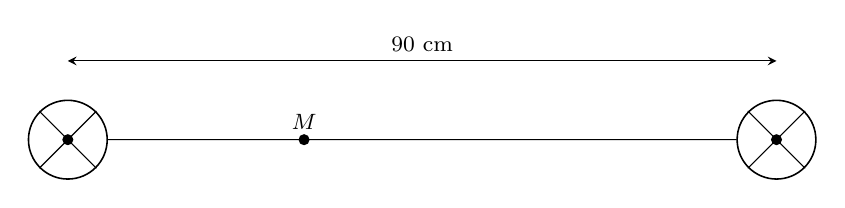
\begin{tikzpicture}[scale=1, font=\footnotesize,line join=round, line cap=round, >=stealth]
			%			\draw[gray,xstep = 1, ystep = 1] (0,0) grid (5,5);
			\path
			(3,0) coordinate (M) node[above] {$M$}
			;
			\node[circle, line width = .2 mm, draw = black, anchor = center, minimum size = 1cm] (D1) at (0,0) {};
			\node[circle, line width = .2 mm, draw = black, anchor = center, minimum size = 1cm] (D2) at (9,0) {};
			
			\draw (D1.0)--(D2.180)
			(D1.45)--(D1.-135)
			(D1.135)--(D1.-45)
			(D2.45)--(D2.-135)
			(D2.135)--(D2.-45)
			;
			\fill
			(D1.center) circle (2pt)
			(D2.center) circle (2pt)
			(M) circle (2pt)
			;
			\draw[stealth-stealth] (0,1) -- (9,1) node[midway,above] {$90$ cm};
		\end{tikzpicture}
	\end{center}
	\shortans{$30$}
	\loigiai{
		Gọi $I$ là cường độ ánh sáng. Vì $I$ tỉ lệ thuận với cường độ của nguồn sáng và tỉ lệ nghịch với bình phương khoảng cách từ điểm đó đến nguồn sáng nên $I=k\dfrac{S}{r^2}$.\\
		Giả sử điểm $M$ nằm cách nguồn sáng $S$ (bên trái) một khoảng là $x$ thì $M$ cách nguồn sáng $8S$ một khoảng là $90-x$.\\
		Ta có cường độ ánh sáng tại điểm $M$ do nguồn sáng $1$ gây ra là $I_1=k\dfrac{S}{x^2}$.\\
		Tương tự cường độ ánh sáng tại điểm $M$ do nguồn sáng $1$ gây ra là $I_1=k\dfrac{8S}{(90-x)^2}$.\\
		Vậy cường độ sáng tổng hợp lại $M$ là
		$$I(x)=I_1+I_2=k\dfrac{S}{x^2}+k\dfrac{8S}{(90-x)^2}$$
		Ta có $I'(x)=-k\dfrac{2Sx}{x^4}-k\dfrac{-16S(90-x)}{(90-x)^4}=kS\left(\dfrac{16}{(90-x)^3}-\dfrac{2}{x^3}\right)$.\\
		$I'(x)=0 \Rightarrow (90-x)^3=8x^3 \Rightarrow 90-x=2x \Rightarrow x=30$ cm.\\
		
		
	}
\end{ex}

\begin{ex}%[2D6V2-3]
	Ở vùng $A$ có hai nhóm, nhóm $1$ là nhóm người có thu nhập tốt (trên $15$ triệu đồng/tháng) và nhóm $2$ là nhóm có thu nhập không tốt. Ở vùng $A$ có $40\%$ người có thu nhập tốt và $58\%$ người không gửi tiết kiệm. Khảo sát độc lập những người thuộc nhóm $1$ và nhóm $2$ và tính tỉ lệ phần trăm số người gửi tiết kiệm của từng nhóm thì thấy rằng: Tỉ lệ người gửi tiết kiệm của nhóm $1$ gấp đôi tỉ lệ người tiết kiệm của nhóm $2$. Giả sử một người ở vùng $A$ không gửi tiết kiệm. Xác suất để người ấy có thu nhập tốt là bao nhiêu $\%$? (kết quả làm tròn đến hàng phần chục).
	
	\shortans{$28$}
	\loigiai{
		Gọi $A$ là biến cố \lq\lq Thu nhập tốt\rq\rq.\\
		Gọi $B$ là biến cố \lq\lq Không gửi tiết kiệm\rq\rq.\\
		Gọi $x$ là tỉ lệ người gửi tiết kiệm ở nhóm $1$, $y$ là tỷ lệ người gửi tiết kiệm ở nhóm $2$.\\
		Theo đề bài ta có $x=2y\quad (1)$.\\
		Gọi $N$ là tổng số người ở vùng $A$, thì số người không gửi tiết kiệm ở nhóm $1$ là $(1-x)\cdot 0{,}4 N$.\\
		Số người không gửi tiết kiệm ở nhóm $2$ là $(1-y)\cdot 0{,}6 N$.\\
		Vì tổng số người không gửi tiết kiệm ở vùng $A$ là $0{,}58N$ nên ta có
		$$(1-x)\cdot 0{,}4 N + (1-y)\cdot 0{,}6 N = 0{,}58N \Leftrightarrow (1-x)\cdot 0{,}4  + (1-y)\cdot 0{,}6  = 0{,}58.\quad(2)$$
		Giải $(1)$ và $(2)$ ta có $x=0{,}6$; $y=0{,}3$.\\
		Theo đề bài ta có
		$P(A)=0{,}4$ và $P(B)=0{,}58$.\\
		Xác suất người không gửi tiết kiệm, biết người đó thu nhập tốt là
		$\mathrm{P}(B\mid A)= 1-0{,}6=0{,}4$.\\
		Vậy xác suất người có thu nhập tốt khi biết người đó không gửi tiết kiệm là
		$$P(A\mid B)=\dfrac{\mathrm{P}(A)\cdot \mathrm{P}(B\mid A)}{\mathrm{P}(B)}=\dfrac{0{,}4\cdot 0{,}4}{0{,}58}=28\%.$$
	}
\end{ex}

\begin{ex}%[2H5V2-7]
	Một radar có thể quay $180^\circ$ để quan sát máy bay quanh vùng phủ sóng của nó. Một máy bay cất cánh từ điểm $A$ nằm trên mặt đất theo chiều cùng chiều với vectơ $\vec{AB}$. Trong hệ tọa độ $Oxyz$ mặt đất là mặt phẳng $(Oxy)$, trục $O z$ hướng lên trời, điểm $A$ nằm trên trục $O y$ cách gốc tọa độ $0{,}6$ km; điểm $B$ nằm trên trục $O z$ có cao độ bằng $0{,}3$ km; radar đang nằm trên trục $Ox$ có hoành độ bằng $0{,}4$ km. Máy bay đang ở điểm $B$ bay theo hướng bay như cũ đến điểm $C(a;b;c)$ thì radar quay một góc bằng $60^\circ$. Tính $a+b+c$ theo đơn vị mét (làm tròn đến hàng đơn vị).
	\begin{center}
		\tikzset{rada/.pic={
				\definecolor{c191716}{RGB}{25,23,22}
				
				\begin{scope}[line cap=round,line join=round]
					\path[fill=white,nonzero rule] (0, 13.21) -- (10.42, 13.21) -- (10.42, 0.02) -- (0, 0.02) --cycle
					(0, 13.21);
					
					\path[fill=white,nonzero rule] (0, 13.21) -- (10.42, 13.21) -- (10.42, 0.02) -- (0, 0.02) --cycle
					(0, 13.21);
					
					\path[fill=c191716,nonzero rule] (0.03, 1.5) .. controls (0, 1.74) and (0.05, 1.99) ..
					(0.18, 2.21) .. controls (0.18, 2.21) and (0.18, 2.21) ..
					(0.18, 2.22) .. controls (0.2, 2.23) and (0.22, 2.23) ..
					(0.24, 2.22) -- (1.73, 0.74) -- (1.73, 0.74) .. controls (1.73, 0.74) and (1.73, 0.73) ..
					(1.73, 0.73) .. controls (1.75, 0.71) and (1.74, 0.69) ..
					(1.72, 0.67) .. controls (1.58, 0.59) and (1.42, 0.54) ..
					(1.25, 0.53) .. controls (1.09, 0.51) and (0.92, 0.53) ..
					(0.77, 0.59) .. controls (0.69, 0.61) and (0.62, 0.65) ..
					(0.55, 0.69) .. controls (0.48, 0.74) and (0.41, 0.79) ..
					(0.35, 0.85) .. controls (0.17, 1.03) and (0.06, 1.26) ..
					(0.03, 1.5);
					
					\path[fill=c191716,even odd rule] (0.39, 0.71) -- (0.06, 0.03) -- (1.2, 0.03) -- (1.2, 0.03) -- (1.22, 0.03) -- (1.04, 0.44) .. controls (0.94, 0.45) and (0.84, 0.47) ..
					(0.74, 0.51) .. controls (0.66, 0.54) and (0.58, 0.58) ..
					(0.5, 0.62) .. controls (0.46, 0.65) and (0.42, 0.68) ..
					(0.39, 0.71);
					
					\path[fill=c191716,even odd rule] (1.21, 1.76) .. controls (1.24, 1.79) and (1.28, 1.79) ..
					(1.31, 1.76) .. controls (1.34, 1.73) and (1.34, 1.69) ..
					(1.31, 1.66) -- (1.03, 1.38) .. controls (1, 1.35) and (0.95, 1.35) ..
					(0.93, 1.38) .. controls (0.9, 1.41) and (0.9, 1.45) ..
					(0.93, 1.48) --
					(1.21, 1.76);
					
					\path[fill=c191716,nonzero rule] (1.33, 1.94) .. controls (1.37, 1.94) and (1.41, 1.92) ..
					(1.45, 1.89) .. controls (1.48, 1.86) and (1.49, 1.82) ..
					(1.49, 1.78) .. controls (1.49, 1.74) and (1.48, 1.7) ..
					(1.45, 1.67) .. controls (1.41, 1.64) and (1.37, 1.62) ..
					(1.33, 1.62) .. controls (1.29, 1.62) and (1.25, 1.64) ..
					(1.22, 1.67) .. controls (1.19, 1.7) and (1.17, 1.74) ..
					(1.17, 1.78) .. controls (1.17, 1.82) and (1.19, 1.86) ..
					(1.22, 1.89) .. controls (1.25, 1.92) and (1.29, 1.94) ..
					(1.33, 1.94);
					
					\path[fill=c191716,even odd rule] (1.49, 2.47) .. controls (1.56, 2.49) and (1.65, 2.49) ..
					(1.72, 2.47) .. controls (1.8, 2.45) and (1.87, 2.42) ..
					(1.93, 2.36) .. controls (1.99, 2.3) and (2.03, 2.23) ..
					(2.05, 2.15) .. controls (2.06, 2.08) and (2.06, 1.99) ..
					(2.04, 1.92) .. controls (2.03, 1.88) and (2.06, 1.84) ..
					(2.1, 1.83) .. controls (2.13, 1.82) and (2.17, 1.85) ..
					(2.18, 1.88) .. controls (2.2, 1.98) and (2.21, 2.09) ..
					(2.18, 2.19) .. controls (2.16, 2.29) and (2.11, 2.38) ..
					(2.03, 2.46) .. controls (1.96, 2.53) and (1.86, 2.58) ..
					(1.76, 2.61) .. controls (1.66, 2.63) and (1.55, 2.63) ..
					(1.45, 2.61) .. controls (1.42, 2.6) and (1.39, 2.56) ..
					(1.4, 2.52) .. controls (1.41, 2.48) and (1.45, 2.46) ..
					(1.49, 2.47) --cycle
					(1.43, 2.26) .. controls (1.49, 2.28) and (1.55, 2.28) ..
					(1.6, 2.26) .. controls (1.66, 2.25) and (1.71, 2.22) ..
					(1.75, 2.18) .. controls (1.8, 2.14) and (1.82, 2.09) ..
					(1.84, 2.03) .. controls (1.85, 1.98) and (1.85, 1.92) ..
					(1.83, 1.86) .. controls (1.83, 1.82) and (1.85, 1.78) ..
					(1.89, 1.78) .. controls (1.93, 1.77) and (1.96, 1.79) ..
					(1.97, 1.83) .. controls (1.99, 1.91) and (1.99, 1.99) ..
					(1.97, 2.07) .. controls (1.96, 2.15) and (1.91, 2.22) ..
					(1.85, 2.28) .. controls (1.79, 2.34) and (1.72, 2.38) ..
					(1.64, 2.4) .. controls (1.56, 2.42) and (1.48, 2.42) ..
					(1.4, 2.4) .. controls (1.36, 2.39) and (1.34, 2.35) ..
					(1.34, 2.32) .. controls (1.35, 2.28) and (1.39, 2.25) ..
					(1.43, 2.26) --cycle
					(1.47, 2) .. controls (1.43, 2) and (1.39, 2.02) ..
					(1.38, 2.06) .. controls (1.38, 2.09) and (1.4, 2.13) ..
					(1.44, 2.14) .. controls (1.47, 2.15) and (1.51, 2.15) ..
					(1.55, 2.14) .. controls (1.59, 2.13) and (1.63, 2.11) ..
					(1.66, 2.08) .. controls (1.68, 2.06) and (1.7, 2.02) ..
					(1.71, 1.98) .. controls (1.72, 1.94) and (1.72, 1.9) ..
					(1.71, 1.87) .. controls (1.7, 1.83) and (1.67, 1.81) ..
					(1.63, 1.82) .. controls (1.59, 1.82) and (1.57, 1.86) ..
					(1.57, 1.9) .. controls (1.58, 1.92) and (1.58, 1.93) ..
					(1.58, 1.95) .. controls (1.57, 1.96) and (1.57, 1.97) ..
					(1.56, 1.98) .. controls (1.54, 1.99) and (1.53, 2) ..
					(1.52, 2.01) .. controls (1.5, 2.01) and (1.49, 2.01) ..
					(1.47, 2);
					
					\path[fill=c191716,even odd rule] (10.37, 13.11) .. controls (10.4, 13.05) and (10.41, 12.96) ..
					(10, 12.72) .. controls (9.98, 12.72) and (9.97, 12.71) ..
					(9.96, 12.7) -- (9.77, 11.86) -- (9.63, 11.78) -- (9.62, 12.52) .. controls (9.39, 12.41) and (9.29, 12.38) ..
					(9.15, 12.33) -- (9.09, 11.97) -- (8.96, 11.9) -- (8.93, 12.27) -- (8.63, 12.48) -- (8.75, 12.56) -- (9.08, 12.43) .. controls (9.2, 12.53) and (9.27, 12.61) ..
					(9.48, 12.74) -- (8.86, 13.12) -- (9, 13.2) -- (9.81, 12.95) .. controls (9.83, 12.96) and (9.84, 12.96) ..
					(9.85, 12.97) .. controls (10.27, 13.21) and (10.34, 13.16) ..
					(10.37, 13.11) --cycle
					(10.37, 13.11);
					
				\end{scope}
				
				
		}}
		\begin{tikzpicture}[scale=.7,transform shape]
			\path (0,0) pic[scale=.3]{rada};
			\path (2.9,2) coordinate (O)
			+(-30:3) coordinate (y) node[above] {$y$}
			+(90:3) coordinate (z) node[above] {$z$}
			+(90:1.8) coordinate (B)
			(.2,0) coordinate (M)
			($(O)!1.3!(M)$) coordinate (x) node[above] {$x$}
			($(O)!-1.5!(y)$) coordinate (y')
			($(O)!-1!(y)$) coordinate (A)
			($(A)!1.5!(B)$) coordinate (v) node[above] {$\overrightarrow{v}$}
			($(A)!1.9!(B)$) coordinate (v')
			;
			%			\draw[gray,xstep = 1, ystep = 1] (0,0) grid (5,5);
			
			\draw[-stealth,dashed] (O)--(z);
			\draw[-stealth,dashed] (O)--(y);
			\draw[-stealth,dashed] (O)--(x);
			\draw[dashed] (O)--(y')
			(A)--(v')
			;
			\draw (0.4,.55)--(B) node[midway,left] {$R$};
			\draw[-stealth] (B)--(v);
			\draw[-stealth] (.5,1) to[bend left = 30] (1.5,0.1) node[right] {$\theta$};
			
			\foreach \x/\g in {B/-45,M/-90,O/-90,A/-90}\fill (\x) circle (1.5pt)+(\g:3mm) node{$\x$};
			
		\end{tikzpicture}
		
	\end{center}
	\shortans{2630}
	\loigiai{
		\begin{center}
			\tikzset{rada/.pic={
					\definecolor{c191716}{RGB}{25,23,22}
					
					\begin{scope}[line cap=round,line join=round]
						\path[fill=white,nonzero rule] (0, 13.21) -- (10.42, 13.21) -- (10.42, 0.02) -- (0, 0.02) --cycle
						(0, 13.21);
						
						\path[fill=white,nonzero rule] (0, 13.21) -- (10.42, 13.21) -- (10.42, 0.02) -- (0, 0.02) --cycle
						(0, 13.21);
						
						\path[fill=c191716,nonzero rule] (0.03, 1.5) .. controls (0, 1.74) and (0.05, 1.99) ..
						(0.18, 2.21) .. controls (0.18, 2.21) and (0.18, 2.21) ..
						(0.18, 2.22) .. controls (0.2, 2.23) and (0.22, 2.23) ..
						(0.24, 2.22) -- (1.73, 0.74) -- (1.73, 0.74) .. controls (1.73, 0.74) and (1.73, 0.73) ..
						(1.73, 0.73) .. controls (1.75, 0.71) and (1.74, 0.69) ..
						(1.72, 0.67) .. controls (1.58, 0.59) and (1.42, 0.54) ..
						(1.25, 0.53) .. controls (1.09, 0.51) and (0.92, 0.53) ..
						(0.77, 0.59) .. controls (0.69, 0.61) and (0.62, 0.65) ..
						(0.55, 0.69) .. controls (0.48, 0.74) and (0.41, 0.79) ..
						(0.35, 0.85) .. controls (0.17, 1.03) and (0.06, 1.26) ..
						(0.03, 1.5);
						
						\path[fill=c191716,even odd rule] (0.39, 0.71) -- (0.06, 0.03) -- (1.2, 0.03) -- (1.2, 0.03) -- (1.22, 0.03) -- (1.04, 0.44) .. controls (0.94, 0.45) and (0.84, 0.47) ..
						(0.74, 0.51) .. controls (0.66, 0.54) and (0.58, 0.58) ..
						(0.5, 0.62) .. controls (0.46, 0.65) and (0.42, 0.68) ..
						(0.39, 0.71);
						
						\path[fill=c191716,even odd rule] (1.21, 1.76) .. controls (1.24, 1.79) and (1.28, 1.79) ..
						(1.31, 1.76) .. controls (1.34, 1.73) and (1.34, 1.69) ..
						(1.31, 1.66) -- (1.03, 1.38) .. controls (1, 1.35) and (0.95, 1.35) ..
						(0.93, 1.38) .. controls (0.9, 1.41) and (0.9, 1.45) ..
						(0.93, 1.48) --
						(1.21, 1.76);
						
						\path[fill=c191716,nonzero rule] (1.33, 1.94) .. controls (1.37, 1.94) and (1.41, 1.92) ..
						(1.45, 1.89) .. controls (1.48, 1.86) and (1.49, 1.82) ..
						(1.49, 1.78) .. controls (1.49, 1.74) and (1.48, 1.7) ..
						(1.45, 1.67) .. controls (1.41, 1.64) and (1.37, 1.62) ..
						(1.33, 1.62) .. controls (1.29, 1.62) and (1.25, 1.64) ..
						(1.22, 1.67) .. controls (1.19, 1.7) and (1.17, 1.74) ..
						(1.17, 1.78) .. controls (1.17, 1.82) and (1.19, 1.86) ..
						(1.22, 1.89) .. controls (1.25, 1.92) and (1.29, 1.94) ..
						(1.33, 1.94);
						
						\path[fill=c191716,even odd rule] (1.49, 2.47) .. controls (1.56, 2.49) and (1.65, 2.49) ..
						(1.72, 2.47) .. controls (1.8, 2.45) and (1.87, 2.42) ..
						(1.93, 2.36) .. controls (1.99, 2.3) and (2.03, 2.23) ..
						(2.05, 2.15) .. controls (2.06, 2.08) and (2.06, 1.99) ..
						(2.04, 1.92) .. controls (2.03, 1.88) and (2.06, 1.84) ..
						(2.1, 1.83) .. controls (2.13, 1.82) and (2.17, 1.85) ..
						(2.18, 1.88) .. controls (2.2, 1.98) and (2.21, 2.09) ..
						(2.18, 2.19) .. controls (2.16, 2.29) and (2.11, 2.38) ..
						(2.03, 2.46) .. controls (1.96, 2.53) and (1.86, 2.58) ..
						(1.76, 2.61) .. controls (1.66, 2.63) and (1.55, 2.63) ..
						(1.45, 2.61) .. controls (1.42, 2.6) and (1.39, 2.56) ..
						(1.4, 2.52) .. controls (1.41, 2.48) and (1.45, 2.46) ..
						(1.49, 2.47) --cycle
						(1.43, 2.26) .. controls (1.49, 2.28) and (1.55, 2.28) ..
						(1.6, 2.26) .. controls (1.66, 2.25) and (1.71, 2.22) ..
						(1.75, 2.18) .. controls (1.8, 2.14) and (1.82, 2.09) ..
						(1.84, 2.03) .. controls (1.85, 1.98) and (1.85, 1.92) ..
						(1.83, 1.86) .. controls (1.83, 1.82) and (1.85, 1.78) ..
						(1.89, 1.78) .. controls (1.93, 1.77) and (1.96, 1.79) ..
						(1.97, 1.83) .. controls (1.99, 1.91) and (1.99, 1.99) ..
						(1.97, 2.07) .. controls (1.96, 2.15) and (1.91, 2.22) ..
						(1.85, 2.28) .. controls (1.79, 2.34) and (1.72, 2.38) ..
						(1.64, 2.4) .. controls (1.56, 2.42) and (1.48, 2.42) ..
						(1.4, 2.4) .. controls (1.36, 2.39) and (1.34, 2.35) ..
						(1.34, 2.32) .. controls (1.35, 2.28) and (1.39, 2.25) ..
						(1.43, 2.26) --cycle
						(1.47, 2) .. controls (1.43, 2) and (1.39, 2.02) ..
						(1.38, 2.06) .. controls (1.38, 2.09) and (1.4, 2.13) ..
						(1.44, 2.14) .. controls (1.47, 2.15) and (1.51, 2.15) ..
						(1.55, 2.14) .. controls (1.59, 2.13) and (1.63, 2.11) ..
						(1.66, 2.08) .. controls (1.68, 2.06) and (1.7, 2.02) ..
						(1.71, 1.98) .. controls (1.72, 1.94) and (1.72, 1.9) ..
						(1.71, 1.87) .. controls (1.7, 1.83) and (1.67, 1.81) ..
						(1.63, 1.82) .. controls (1.59, 1.82) and (1.57, 1.86) ..
						(1.57, 1.9) .. controls (1.58, 1.92) and (1.58, 1.93) ..
						(1.58, 1.95) .. controls (1.57, 1.96) and (1.57, 1.97) ..
						(1.56, 1.98) .. controls (1.54, 1.99) and (1.53, 2) ..
						(1.52, 2.01) .. controls (1.5, 2.01) and (1.49, 2.01) ..
						(1.47, 2);
						
						\path[fill=c191716,even odd rule] (10.37, 13.11) .. controls (10.4, 13.05) and (10.41, 12.96) ..
						(10, 12.72) .. controls (9.98, 12.72) and (9.97, 12.71) ..
						(9.96, 12.7) -- (9.77, 11.86) -- (9.63, 11.78) -- (9.62, 12.52) .. controls (9.39, 12.41) and (9.29, 12.38) ..
						(9.15, 12.33) -- (9.09, 11.97) -- (8.96, 11.9) -- (8.93, 12.27) -- (8.63, 12.48) -- (8.75, 12.56) -- (9.08, 12.43) .. controls (9.2, 12.53) and (9.27, 12.61) ..
						(9.48, 12.74) -- (8.86, 13.12) -- (9, 13.2) -- (9.81, 12.95) .. controls (9.83, 12.96) and (9.84, 12.96) ..
						(9.85, 12.97) .. controls (10.27, 13.21) and (10.34, 13.16) ..
						(10.37, 13.11) --cycle
						(10.37, 13.11);
						
					\end{scope}
					
					
			}}
			\begin{tikzpicture}[scale=.7,transform shape]
				\path (0,0) pic[scale=.3]{rada};
				\path (2.9,2) coordinate (O)
				+(-30:3) coordinate (y) node[above] {$y$}
				+(90:3) coordinate (z) node[above] {$z$}
				+(90:1.8) coordinate (B)
				(.2,0) coordinate (M)
				($(O)!1.3!(M)$) coordinate (x) node[above] {$x$}
				($(O)!-1.5!(y)$) coordinate (y')
				($(O)!-1!(y)$) coordinate (A)
				($(A)!1.5!(B)$) coordinate (v) node[above] {$\overrightarrow{v}$}
				($(A)!1.9!(B)$) coordinate (v') node[above] {$C$}
				;
				%			\draw[gray,xstep = 1, ystep = 1] (0,0) grid (5,5);
				
				\draw[-stealth,dashed] (O)--(z);
				\draw[-stealth,dashed] (O)--(y);
				\draw[-stealth,dashed] (O)--(x);
				\draw[dashed] (O)--(y')
				(A)--(v')
				(M)--(v')
				;
				\draw (0.4,.55)--(B) node[midway,left] {$R$};
				\draw[-stealth] (B)--(v);
				%			\draw[-stealth] (.5,1) to[bend left = 30] (1.5,0.1) node[right] {$\theta$};
				
				\foreach \x/\g in {B/-45,M/-90,O/-90,A/-90}\fill (\x) circle (1.5pt)+(\g:3mm) node{$\x$}
				;
				\fill (v') circle(1.5pt);
				\draw[thin,fill=gray] pic[angle radius = 40pt, "$60^\circ$", angle eccentricity = 1.3]{ angle = v'--M--B};
			\end{tikzpicture}
		\end{center}
		Ta có điểm $A(0;-0{,}6;0)$; $B(0;0;0{,}3)$, $M(0{,}4;0;0)$.\\
		Vậy $\overrightarrow{AB}=(0;0{,}6;0{,}3)$ nên véctơ $\overrightarrow{u}=(0;2;1)$.\\
		Do đó phương trình đường thẳng $AB$ là $\heva{&x=0\\&y=2t\\&z=0{,}3t.}$\\
		Điểm $C$ thuộc đường thẳng $AB$ nên có tọa độ là $C(0;2t;0{,}3t)$.
		Vì $C$ ứng với góc quay $60^\circ$ của radar nên $\widehat{BMC}=60^\circ$.\\
		$\overrightarrow{MB}=(-0{,}4;0;0{,}3)$; $\overrightarrow{MC}=(-0{,}4;2t;0{,}3+t)$.\\
		Ta có $$\cos \widehat{BMC}=\dfrac{\overrightarrow{MB}\cdot \overrightarrow{MC}}{\left|\overrightarrow{MB}\right|\cdot \left|\overrightarrow{MC}\right|}=\dfrac{0{,}25+0{,}3t}{0{,}5\cdot \sqrt{5t^2+0{,}6t+0{,}25}}=\dfrac{1}{2}.\quad (*)$$
		Rút gọn $(*)$ ta thu được phương trình bậc hai
		$$
		3{,}56t^2-1{,}8t-0{,}75=0.
		$$
		Phương trình trên có hai nghiệm là $t\approx -0{,}27120$ (loại) và $t\approx 0{,}776819$.\\
		Vậy $a+b+c=0+2t+0{,}3+t=0{,}3+3t=2{,630457}$ (km) $\approx 2630$ (m).
	}
\end{ex}
\Closesolutionfile{ans}